\documentclass[11pt,a4paper]{article}

% ------------------------------------------------------------
% Packages
% ------------------------------------------------------------
\usepackage[margin=1in]{geometry}
\usepackage{amsmath,amssymb,bm}
\usepackage{graphicx}
% search paths for included graphics (try both figures/ and images/)
% include parent-folder figures/ where the project's figures live
\graphicspath{{../figures/}{figures/}{images/}{./}}
\usepackage{booktabs}
\usepackage{array}
\usepackage{siunitx}
\usepackage{float}
\usepackage{caption}
\usepackage{subcaption}
\usepackage{hyperref}
\usepackage{xcolor}

\sisetup{
        round-mode=places,
        round-precision=3,
        detect-all
}

% ------------------------------------------------------------
% Convenience macros (from user's past document)
% ------------------------------------------------------------
\newcommand{\dd}{\,\mathrm{d}}
\newcommand{\grad}{\nabla}
\newcommand{\vect}[1]{\begin{Bmatrix}#1\end{Bmatrix}}
\newcommand{\mat}[1]{\begin{bmatrix}#1\end{bmatrix}}

% Header/footer style
\usepackage{fancyhdr}
\fancyhf{}
\fancyhead[L]{CE586 Assignment 4}
\fancyhead[R]{Imran Shahriar - 2735835}
\renewcommand{\headrulewidth}{0.4pt}
\fancyfoot[C]{\thepage}
\fancypagestyle{plain}{%
    \fancyhf{}
    \fancyhead[L]{CE586 Assignment 4}
    \fancyhead[R]{Imran Shahriar - 2735835}
    \renewcommand{\headrulewidth}{0.4pt}
    \fancyfoot[C]{\thepage}}
\pagestyle{fancy}

\hypersetup{
    colorlinks=true,
    linkcolor=blue,
    citecolor=blue,
    urlcolor=blue
}

\begin{document}

% ============================================================
% Title Page
% ============================================================
\begin{titlepage}
    \begin{flushright}
        {\large \today\par}
    \end{flushright}

    \vspace*{0.5cm}

    \begin{center}
        
\includegraphics[width=0.42\textwidth]{../figures/metu_logo.jpg}\par
        \vspace{0.7cm}
        {\huge CE586 Assignment 4\par}
        \vspace{0.3cm}
        {\Large Earthquake Engineering\par}
        \vspace{0.45cm}
        {\Large Spring Semester 2025--2026\par}
 \vspace{0.45cm}
\end{center}

\vspace{0.9cm}

\noindent
\begin{minipage}[t]{0.48\textwidth}
    \raggedright
    {\Large \textbf{Submitted By}\par}
    \vspace{0.3cm}
    {\large Imran Shahriar\par}
    \vspace{0.2cm}
    {\large 2735835\par}
    \vspace{0.2cm}
    {\large MSc. in Structural Engineering\par}
\end{minipage}
\hfill
\begin{minipage}[t]{0.48\textwidth}
    \raggedleft
    {\Large \textbf{Submitted To}\par}
    \vspace{0.3cm}
    {\large Prof. MURAT ALTUĞ ERBERİK\par}
\end{minipage}

\vspace{0.5cm}

\begin{center}
\textbf{\large GitHub Repository:} 
\href{https://github.com/ImranMETU/CE586_Assignment4}{\url{https://github.com/ImranMETU/CE586_Assignment4}}
\end{center}
    \vfill
\end{titlepage}
\hypersetup{pageanchor=true}

\tableofcontents
\pagebreak
\section{Introduction and Given Data}

This report presents the dynamic analysis of a three-story shear-frame building subjected to the DIN95Y01 horizontal ground-motion record. The assignment is solved in four stages. First, the equation of motion is obtained for two structural idealizations: flexurally rigid beams and beams with finite flexural stiffness. For the finite-beam case, static condensation is used to eliminate rotational degrees of freedom and retain only the lateral floor displacements. Second, eigenvalue analysis is carried out for the undamped flexurally rigid-beam model. Third, modal response history analysis is performed using the assigned ground-motion record. Finally, a 5\% elastic response spectrum is constructed and used for response spectrum analysis with ABSSUM, SRSS, and CQC modal combination rules. The equivalent static lateral force procedure is also applied using the prescribed design spectrum. \\
The structure considered in this assignment is a three-story idealized frame building. The columns are assumed massless, and the floor masses are lumped at the story levels. Axial deformations are neglected. The horizontal ground acceleration is denoted by $\ddot{u}_g(t)$.

The lateral degrees of freedom are selected as
\begin{equation}
\bm{u}(t)=
\begin{bmatrix}
 u_1(t)\\
 u_2(t)\\
 u_3(t)
\end{bmatrix},
\end{equation}
where $u_i(t)$ is the lateral displacement of floor $i$ relative to the ground.

The given properties are
\begin{equation}
EI=3600\ \mathrm{kN\,m^2},
\qquad h=3\ \mathrm{m},
\qquad L_b=4\ \mathrm{m},
\end{equation}
where $h$ is the story height and $L_b$ is the beam span. The floor masses are
\begin{equation}
 m_1=20\ \mathrm{t},\qquad m_2=15\ \mathrm{t},\qquad m_3=15\ \mathrm{t}.
\end{equation}
Therefore, the mass matrix is
\begin{equation}
\bm{M}=\begin{bmatrix}
20&0&0\\
0&15&0\\
0&0&15
\end{bmatrix}\ \mathrm{t}.
\end{equation}

The influence vector for horizontal base excitation is
\begin{equation}
\bm{1}=\begin{bmatrix}1\\1\\1\end{bmatrix}.
\end{equation}

The general equation of motion for the lateral degrees of freedom is
\begin{equation}
\boxed{
\bm{M}\ddot{\bm{u}}(t)+\bm{C}\dot{\bm{u}}(t)+\bm{K}\bm{u}(t)
=-\bm{M}\bm{1}\ddot{u}_g(t)
}
\end{equation}
\pagebreak
\section{Q1: Equation of Motion for Two Beam Idealizations}
\subsection{Case 1: Flexurally Rigid}
For the flexurally rigid-beam idealization, the story stiffness coefficients are
\begin{equation}
k_1=6400\ \mathrm{kN/m},
\qquad
k_2=6400\ \mathrm{kN/m},
\qquad
k_3=3200\ \mathrm{kN/m}.
\end{equation}

The per-story lateral stiffness used in the rigid-beam idealization is formed from the elastic flexural stiffness of the vertical elements. Following the finite-beam partition and condensation used elsewhere in this assignment, the contribution for a single story segment (with height $h$ and flexural rigidity $EI$) leads to an elementary rotational stiffness term
\begin{equation}
k_{\mathrm{elem}}=\frac{12\,EI}{h^3}\ \mathrm{(kN/m)}.
\end{equation}
\begin{equation}
k_i = 2\,n_i\,k_{\mathrm{elem}},
\end{equation}
where $n_i$ is the factor accounting for the effective flexural subsystem used in the assembly ($n_1=n_2=1$ for the lower two stories with two-legged contribution, and $n_3=\tfrac{1}{2}$ for the top story in this modelling choice). Substituting the given $EI=3600\ \mathrm{kN\,m^2}$ and $h=3\ \mathrm{m}$:
\begin{align}
k_{\mathrm{elem}} &= \frac{12(3600)}{3^3} = \frac{43200}{27} = 1600\ \mathrm{kN/m},\\
k_1 &= 2\times(2)\times1600 = 6400\ \mathrm{kN/m},\\
k_2 &= 2\times(2)\times1600 = 6400\ \mathrm{kN/m},\\
k_3 &= 2\times(1)\times1600 = 3200\ \mathrm{kN/m}.
\end{align}

These values are then assembled into the standard three-story rigid-beam stiffness matrix by placing the story stiffnesses on the diagonal and using the convention of negative off-diagonal coupling between adjacent degrees of freedom:
\begin{equation}
\boxed{\bm{K}_r=\begin{bmatrix}
k_1+k_2 & -k_2 & 0\\
-k_2 & k_2+k_3 & -k_3\\
0 & -k_3 & k_3
\end{bmatrix}}
\end{equation}
Substituting the computed $k_i$ yields
\begin{equation}
\boxed{\bm{K}_r=\begin{bmatrix}
12800 & -6400 & 0\\
-6400 & 9600 & -3200\\
0 & -3200 & 3200
\end{bmatrix}\ \mathrm{kN/m}.}
\end{equation}
The assembled rigid-beam stiffness matrix is
\begin{equation}
\boxed{
\bm{K}_r=
\begin{bmatrix}
12800 & -6400 & 0\\
-6400 & 9600 & -3200\\
0 & -3200 & 3200
\end{bmatrix}
\ \mathrm{kN/m}
}
\label{eq:Kr}
\end{equation}
and the rigid-beam equation of motion is
\begin{equation}
\bm{M}\ddot{\bm{u}}(t)+\bm{K}_r\bm{u}(t)
=-\bm{M}\bm{1}\ddot{u}_g(t).
\end{equation}

For Case 1, Rayleigh damping is obtained by enforcing $\xi_1=\xi_2=0.05$ on the first two rigid-beam modes. Using $\omega_1=8.573542\ \mathrm{rad/s}$ and $\omega_2=19.537283\ \mathrm{rad/s}$ from eigenvalue analysis in Q2,
\begin{equation}
\begin{bmatrix}
\frac{1}{2\omega_1} & \frac{\omega_1}{2}\\
\frac{1}{2\omega_2} & \frac{\omega_2}{2}
\end{bmatrix}
\begin{bmatrix}
a_0\\
a_1
\end{bmatrix}
=
\begin{bmatrix}
0.05\\
0.05
\end{bmatrix}.
\end{equation}
Solving gives
\begin{equation}
\boxed{a_0=0.595869},
\qquad
\boxed{a_1=0.003557}.
\end{equation}
Hence the Case 1 damping matrix is
\begin{equation}
\bm{C}_r=a_0\bm{M}+a_1\bm{K}_r.
\end{equation}

Numerically,
\begin{equation}
\bm{C}_r=
\begin{bmatrix}
57.446980 & -22.764800 & 0.000000\\
-22.764800 & 43.085235 & -11.382400\\
0.000000 & -11.382400 & 20.320435
\end{bmatrix}
\ \mathrm{kN\,s/m}.
\end{equation} Thus, the equation of motion for the flexurally rigid-beam model is

\begin{equation}
\boxed{
\bm{M}\ddot{\bm{u}}+\bm{C}_r\dot{\bm{u}}+\bm{K}_r\bm{u}
=-\bm{M}\bm{1}\ddot{u}_g(t)
}
\label{eq:eom_rigid}
\end{equation}

Thus, the assembled matrix form of the rigid-beam equation of motion (with numerical damping) is
\begin{equation}
\boxed{%
\begin{aligned}
&\begin{bmatrix}20 & 0 & 0\\ 0 & 15 & 0\\ 0 & 0 & 15\end{bmatrix}\,\ddot{\bm{u}}(t)
+\begin{bmatrix}57.446980 & -22.764800 & 0.000000\\ -22.764800 & 43.085235 & -11.382400\\ 0.000000 & -11.382400 & 20.320435\end{bmatrix}\,\dot{\bm{u}}(t)\\[4pt]
&\quad +\begin{bmatrix}12800 & -6400 & 0\\ -6400 & 9600 & -3200\\ 0 & -3200 & 3200\end{bmatrix}\,\bm{u}(t)\\[6pt]
&= -\begin{bmatrix}20 & 0 & 0\\ 0 & 15 & 0\\ 0 & 0 & 15\end{bmatrix}\,\bm{1}\,\ddot{u}_g(t)
\end{aligned}%
}
\label{eq:M}
\end{equation}

\pagebreak
\subsection{Case 2: Flexural Stiffness EI}
For the finite-beam case, the global stiffness matrix is partitioned into translational and rotational degrees of freedom. Static condensation gives
\begin{equation}
\bm{s}=-\bm{K}_{ss}^{-1}\bm{K}_{sd}\bm{d}.
\end{equation}
Substituting into the lateral equilibrium equation gives the condensed lateral stiffness matrix
\begin{equation}
\boxed{
\bm{K}_c=\bm{K}_{dd}-\bm{K}_{ds}\bm{K}_{ss}^{-1}\bm{K}_{sd}
}
\label{eq:condensation}
\end{equation}

The resulting condensed stiffness matrix is
\begin{equation}
\boxed{
\bm{K}_c=
\begin{bmatrix}
10281.790 & -5335.993 & 962.845\\
-5335.993 & 6147.848 & -2477.414\\
962.845 & -2477.414 & 1702.442
\end{bmatrix}\ \mathrm{kN/m}
}
\label{eq:Kc}
\end{equation}

\subsubsection*{Finite-beam partition matrices and numeric condensation}
The finite-beam model used a larger stiffness matrix partitioned into translational DOFs (the retained lateral displacements) and rotational/internal DOFs. The Python implementation produced the following numeric partitions (units: kN/m):

\begin{equation}
\bm{K}_{dd}=\begin{bmatrix}
12800.000 & -6400.000 & 0.000\\
-6400.000 & 9600.000 & -3200.000\\
0.000 & -3200.000 & 3200.000
\end{bmatrix}
\end{equation}

\begin{equation}
\bm{K}_{ds}=\begin{bmatrix}
0.000 & 0.000 & 4800.000 & 4800.000 & 0.000 & 0.000\\
-4800.000 & -4800.000 & -2400.000 & -2400.000 & 2400.000 & 2400.000\\
0.000 & 0.000 & -2400.000 & -2400.000 & -2400.000 & -2400.000
\end{bmatrix}
\end{equation}

\begin{equation}
\bm{K}_{ss}=\begin{bmatrix}
22800.000 & 1800.000 & 4800.000 & 0.000 & 0.000 & 0.000\\
1800.000 & 22800.000 & 0.000 & 4800.000 & 0.000 & 0.000\\
4800.000 & 0.000 & 18000.000 & 1800.000 & 2400.000 & 0.000\\
0.000 & 4800.000 & 1800.000 & 18000.000 & 0.000 & 2400.000\\
0.000 & 0.000 & 2400.000 & 0.000 & 8400.000 & 1800.000\\
0.000 & 0.000 & 0.000 & 2400.000 & 1800.000 & 8400.000
\end{bmatrix}
\end{equation}

The condensation step computes
\begin{equation}
\bm{K}_c=\bm{K}_{dd}-\bm{K}_{ds}\bm{K}_{ss}^{-1}\bm{K}_{sd}.
\end{equation}

Python computed the intermediate product \(\bm{K}_{ds}\bm{K}_{ss}^{-1}\bm{K}_{sd}\) as
\begin{equation}
\begin{bmatrix}
2518.210 & -1064.007 & -962.845\\
-1064.007 & 3452.152 & -722.586\\
-962.845 & -722.586 & 1497.558
\end{bmatrix}
\end{equation}

Subtracting this from $\bm{K}_{dd}$ yields the condensed stiffness
\begin{equation}
\boxed{\bm{K}_c=\begin{bmatrix}
10281.790 & -5335.993 & 962.845\\
-5335.993 & 6147.848 & -2477.414\\
962.845 & -2477.414 & 1702.442
\end{bmatrix}\ \mathrm{kN/m}}
\end{equation}

These numeric partitions and intermediate results were generated by the function \texttt{build\_finite\_beam\_condensed\_stiffness()} in \texttt{Q3.py} and are consistent with the condensed matrix used elsewhere in this report.

The first two natural circular frequencies of the condensed model are
\begin{equation}
\omega_1=4.554048\ \mathrm{rad/s},
\qquad
\omega_2=14.479587\ \mathrm{rad/s}.
\end{equation}
Using Rayleigh damping with $\xi_1=\xi_2=0.05$ gives
\begin{equation}
\boxed{a_0=0.346443},
\qquad
\boxed{a_1=0.005254}.
\end{equation}
Thus,
\begin{equation}
\boxed{
\bm{C}_c=
\begin{bmatrix}
60.948 & -28.035 & 5.059\\
-28.035 & 37.497 & -13.016\\
5.059 & -13.016 & 14.141
\end{bmatrix}\ \mathrm{kN\,s/m}
}
\label{eq:Cc}
\end{equation}

The equation of motion for the finite-beam model after static condensation is
\begin{equation}
\boxed{
\bm{M}\ddot{\bm{u}}+\bm{C}_c\dot{\bm{u}}+\bm{K}_c\bm{u}
=-\bm{M}\bm{1}\ddot{u}_g(t)
}
\label{eq:eom_condensed}
\end{equation}

\subsection{Comparison of the Two Beam Idealizations}

\begin{table}[H]
\centering
\caption{Comparison of natural periods for the two beam idealizations.}
\begin{tabular}{cccc}
\toprule
Mode & $T_n$ rigid beams (s) & $T_n$ finite beams (s) & Observation\\
\midrule
1 & 0.733 & 1.380 & finite beams significantly increase flexibility\\
2 & 0.322 & 0.434 & finite beams increase period\\
3 & 0.195 & 0.221 & smaller but visible increase\\
\bottomrule
\end{tabular}
\label{tab:q1_period_comparison}
\end{table}

The finite-beam model is more flexible than the flexurally rigid-beam model because joint rotations are allowed. Consequently, the condensed lateral stiffness matrix is softer, and the natural periods increase. The rigid-beam idealization therefore gives a stiffer shear-building approximation.
\pagebreak
% ------------------------------------------------------------
\section{Q2: Undamped Eigenvalue Analysis for Flexurally Rigid Beams}
% ------------------------------------------------------------

For the undamped flexurally rigid-beam model,
\begin{equation}
\bm{C}=\bm{0},
\end{equation}
and the free-vibration equation is
\begin{equation}
\bm{M}\ddot{\bm{u}}+\bm{K}_r\bm{u}=\bm{0}.
\end{equation}
Assuming harmonic motion,
\begin{equation}
\bm{u}(t)=\bm{\phi}e^{i\omega t},
\end{equation}
leads to
\begin{equation}
\bm{K}_r\bm{\phi}=\omega^2\bm{M}\bm{\phi}.
\end{equation}
Let
\begin{equation}
\lambda=\omega^2.
\end{equation}
Then the eigenvalue problem becomes
\begin{equation}
(\bm{K}_r-\lambda\bm{M})\bm{\phi}=\bm{0}.
\end{equation}
For a non-trivial mode shape,
\begin{equation}
\boxed{\det(\bm{K}_r-\lambda\bm{M})=0}
\end{equation}

Using $\bm{K}_r$ and $\bm{M}$,
\begin{equation}
\bm{K}_r-\lambda\bm{M}=
\begin{bmatrix}
12800-20\lambda & -6400 & 0\\
-6400 & 9600-15\lambda & -3200\\
0 & -3200 & 3200-15\lambda
\end{bmatrix}.
\end{equation}
The determinant gives
\begin{equation}
\det(\bm{K}_r-\lambda\bm{M})=
-4500\lambda^3
+6720000\lambda^2
-2252800000\lambda
+131072000000.
\end{equation}
Therefore, the characteristic equation is
\begin{equation}
\boxed{
-4500\lambda^3
+6720000\lambda^2
-2252800000\lambda
+131072000000=0
}
\label{eq:characteristic}
\end{equation}
Equivalently,
\begin{equation}
9\lambda^3-13440\lambda^2+4505600\lambda-262144000=0.
\end{equation}

Solving Eq.~\eqref{eq:characteristic}, the eigenvalues are
\begin{equation}
\lambda_1=73.505625,
\qquad
\lambda_2=381.705412,
\qquad
\lambda_3=1038.122296.
\end{equation}
Since $\lambda_n=\omega_n^2$,
\begin{equation}
\omega_1=8.573542\ \mathrm{rad/s},
\qquad
\omega_2=19.537283\ \mathrm{rad/s},
\qquad
\omega_3=32.219905\ \mathrm{rad/s}.
\end{equation}
The natural periods are
\begin{equation}
T_n=\frac{2\pi}{\omega_n},
\end{equation}
which gives
\begin{equation}
T_1=0.732858\ \mathrm{s},
\qquad
T_2=0.321600\ \mathrm{s},
\qquad
T_3=0.195009\ \mathrm{s}.
\end{equation}

The roof-normalized mode shape matrix is
\begin{equation}
\boxed{
\bm{\Phi}=
\begin{bmatrix}
0.370245 & -0.977791 & 3.107546\\
0.655442 & -0.789244 & -3.866198\\
1.000000 & 1.000000 & 1.000000
\end{bmatrix}
}
\label{eq:Phi}
\end{equation}
where each column corresponds to one mode shape.

\begin{table}[H]
\centering
\caption{Undamped eigenvalue analysis results for the flexurally rigid-beam model.}
\begin{tabular}{cccc}
\toprule
Mode & $\lambda_n=\omega_n^2$ $(\mathrm{s^{-2}})$ & $\omega_n$ $(\mathrm{rad/s})$ & $T_n$ (s)\\
\midrule
1 & 73.505625 & 8.573542 & 0.732858\\
2 & 381.705412 & 19.537283 & 0.321600\\
3 & 1038.122296 & 32.219905 & 0.195009\\
\bottomrule
\end{tabular}
\label{tab:q2_eigenvalues}
\end{table}
\pagebreak
% ------------------------------------------------------------
\section{Q3: Response History Analysis}
% ------------------------------------------------------------

\subsection{Modal Properties}
The modal participation quantities are defined as
\begin{equation}
L_n=\bm{\phi}_n^T\bm{M}\bm{1},
\end{equation}
\begin{equation}
M_n=\bm{\phi}_n^T\bm{M}\bm{\phi}_n,
\end{equation}
and
\begin{equation}
\Gamma_n=\frac{L_n}{M_n}.
\end{equation}

Using the roof-normalized mode shapes from Eq.~\eqref{eq:Phi}, the modal properties are summarized in Table~\ref{tab:q3_modal_properties}.

\begin{table}[H]
\centering
\caption{Modal participation quantities.}
\begin{tabular}{cccc}
\toprule
Mode & $L_n$ (t) & $M_n$ (t) & $\Gamma_n$\\
\midrule
1 & 32.237 & 24.186 & 1.333\\
2 & -16.394 & 43.465 & -0.377\\
3 & 19.158 & 432.349 & 0.044\\
\bottomrule
\end{tabular}
\label{tab:q3_modal_properties}
\end{table}

\subsection{Modal SDOF Response Histories}

For each mode, the uncoupled modal equation is
\begin{equation}
\ddot{D}_n(t)+2\xi_n\omega_n\dot{D}_n(t)+\omega_n^2D_n(t)
=-\ddot{u}_g(t).
\end{equation}
The DIN95Y01 ground motion record was used as the excitation. The record contains 2796 points with $\Delta t=0.01\ \mathrm{s}$ and a PGA of $313.190\ \mathrm{cm/s^2}=0.3194g$.

The maximum modal displacement responses $D_n(t)$ are given in Table~\ref{tab:q3_Dn}.

\begin{table}[H]
\centering
\caption{Maximum modal SDOF displacement responses $D_n(t)$.}
\begin{tabular}{ccccc}
\toprule
Mode & $T_n$ (s) & $\xi_n$ & $\max|D_n|$ (m) & Time (s)\\
\midrule
1 & 0.733 & 0.0500 & 0.05317 & 9.58\\
2 & 0.322 & 0.0500 & 0.03115 & 4.45\\
3 & 0.195 & 0.0666 & 0.00641 & 3.73\\
\bottomrule
\end{tabular}
\label{tab:q3_Dn}
\end{table}

\begin{figure}[H]
\centering
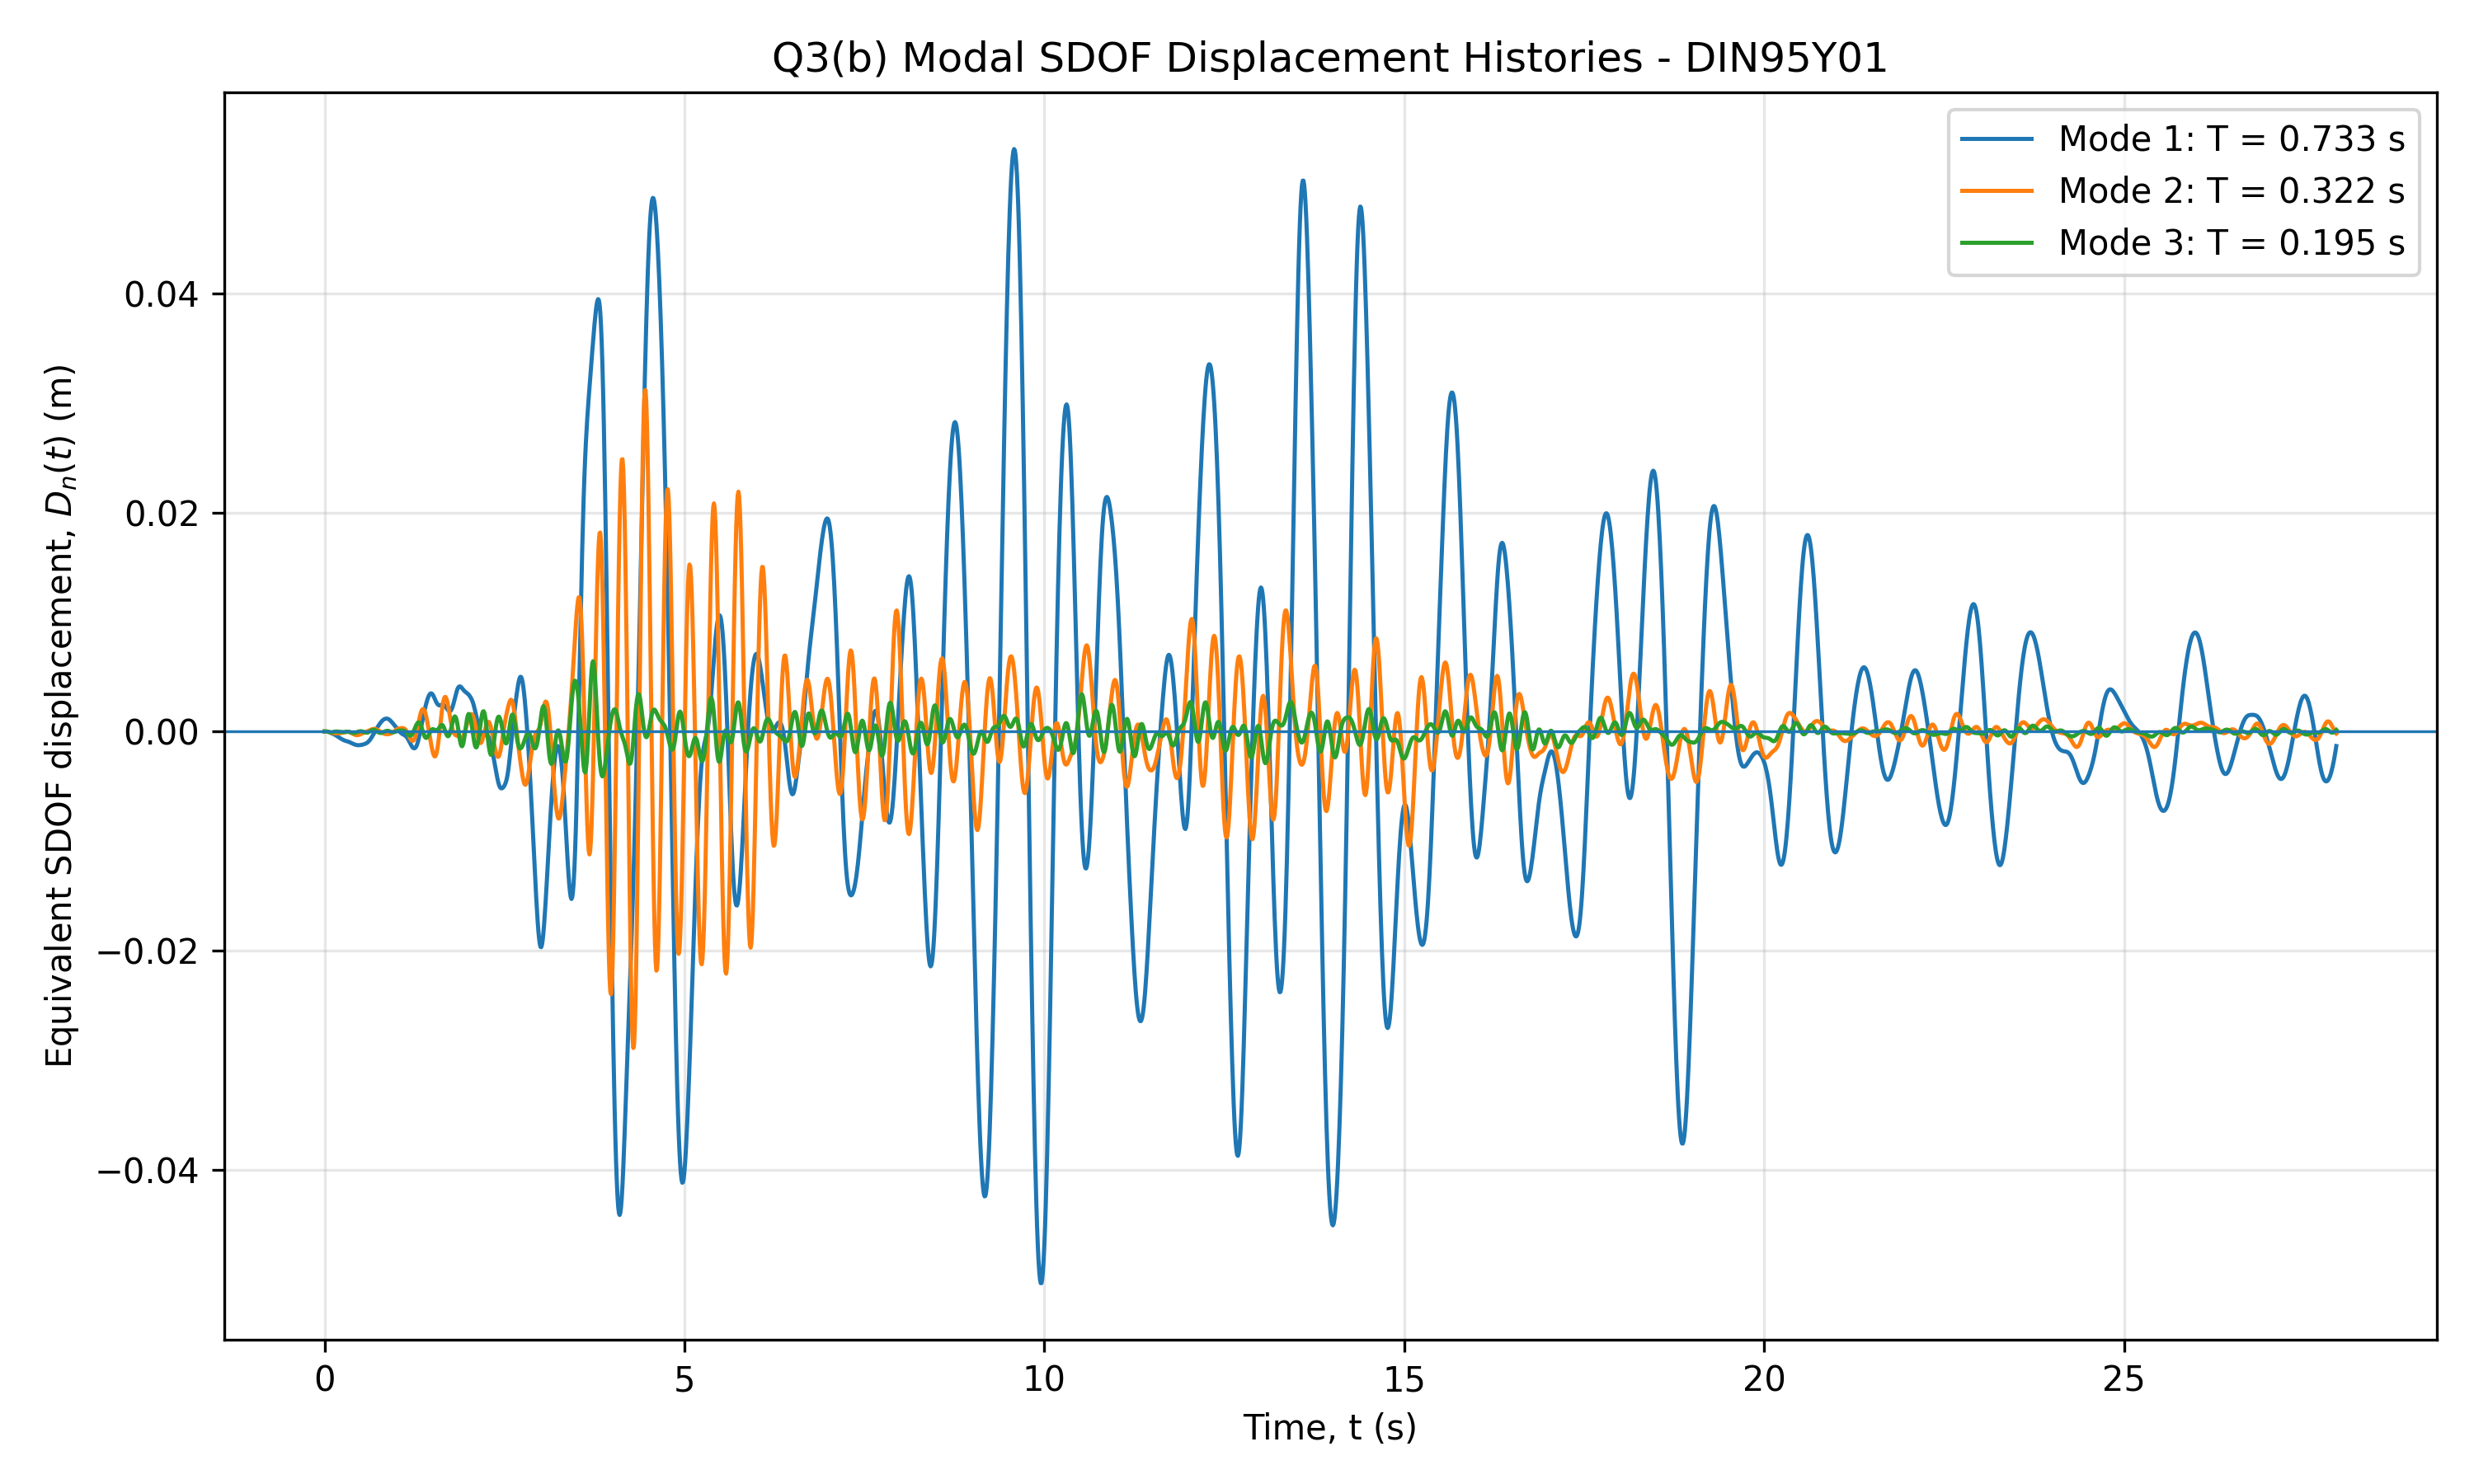
\includegraphics[width=0.92\textwidth]{../figures/Q3b_modal_SDOF_displacement_histories.png}
\caption{Modal SDOF displacement histories $D_n(t)$.}
\label{fig:q3b_modal_histories}
\end{figure}

\subsection{Floor Displacements and Story Drifts}

The floor displacement vector is reconstructed by modal superposition:
\begin{equation}
\bm{u}(t)=\sum_{n=1}^{3}\bm{\phi}_n\Gamma_nD_n(t).
\end{equation}


For each mode $n$, the modal displacement contribution is
\begin{equation}
\mathbf{u}_n(t)=\boldsymbol{\phi}_n\Gamma_nD_n(t).
\end{equation}

\begin{equation}
\boldsymbol{\phi}_1\Gamma_1=
\begin{bmatrix}
0.493490\\
0.873623\\
1.332876
\end{bmatrix},
\qquad
\boldsymbol{\phi}_2\Gamma_2=
\begin{bmatrix}
0.368810\\
0.297693\\
-0.377187
\end{bmatrix},
\qquad
\boldsymbol{\phi}_3\Gamma_3=
\begin{bmatrix}
0.137699\\
-0.171316\\
0.044311
\end{bmatrix}.
\end{equation}

\begin{equation}
\mathbf{u}_1(t)=
\begin{bmatrix}
0.493490\\
0.873623\\
1.332876
\end{bmatrix}
D_1(t),
\end{equation}
\begin{equation}
\mathbf{u}_2(t)=
\begin{bmatrix}
0.368810\\
0.297693\\
-0.377187
\end{bmatrix}
D_2(t),
\end{equation}
\begin{equation}
\mathbf{u}_3(t)=
\begin{bmatrix}
0.137699\\
-0.171316\\
0.044311
\end{bmatrix}
D_3(t).
\end{equation}

The total displacement vector is
\begin{equation}
\mathbf{u}(t)=\mathbf{u}_1(t)+\mathbf{u}_2(t)+\mathbf{u}_3(t).
\end{equation}

Expanded floor by floor,
\begin{equation}
u_1(t)=0.493490D_1(t)+0.368810D_2(t)+0.137699D_3(t),
\end{equation}
\begin{equation}
u_2(t)=0.873623D_1(t)+0.297693D_2(t)-0.171316D_3(t),
\end{equation}
\begin{equation}
u_3(t)=1.332876D_1(t)-0.377187D_2(t)+0.044311D_3(t).
\end{equation}

These expressions provide the direct modal superposition form used in the response-history reconstruction.

The story drifts are
\begin{equation}
\Delta_1=u_1,
\qquad
\Delta_2=u_2-u_1,
\qquad
\Delta_3=u_3-u_2.
\end{equation}

\begin{table}[H]
\centering
\caption{Maximum floor displacements.}
\begin{tabular}{cccc}
\toprule
Floor & $\max|u_i|$ (m) & Time (s) & Signed value (m)\\
\midrule
1 & 0.02983 & 4.48 & 0.02983\\
2 & 0.04795 & 9.57 & 0.04795\\
3 & 0.07121 & 4.59 & 0.07121\\
\bottomrule
\end{tabular}
\label{tab:q3_floor_displacements}
\end{table}

\begin{table}[H]
\centering
\caption{Maximum story drifts.}
\begin{tabular}{cccc}
\toprule
Story & Drift definition & $\max|\Delta_i|$ (m) & Time (s)\\
\midrule
1 & $u_1$ & 0.02983 & 4.48\\
2 & $u_2-u_1$ & 0.01962 & 13.59\\
3 & $u_3-u_2$ & 0.03641 & 4.61\\
\bottomrule
\end{tabular}
\label{tab:q3_drifts}
\end{table}

\begin{figure}[H]
\centering
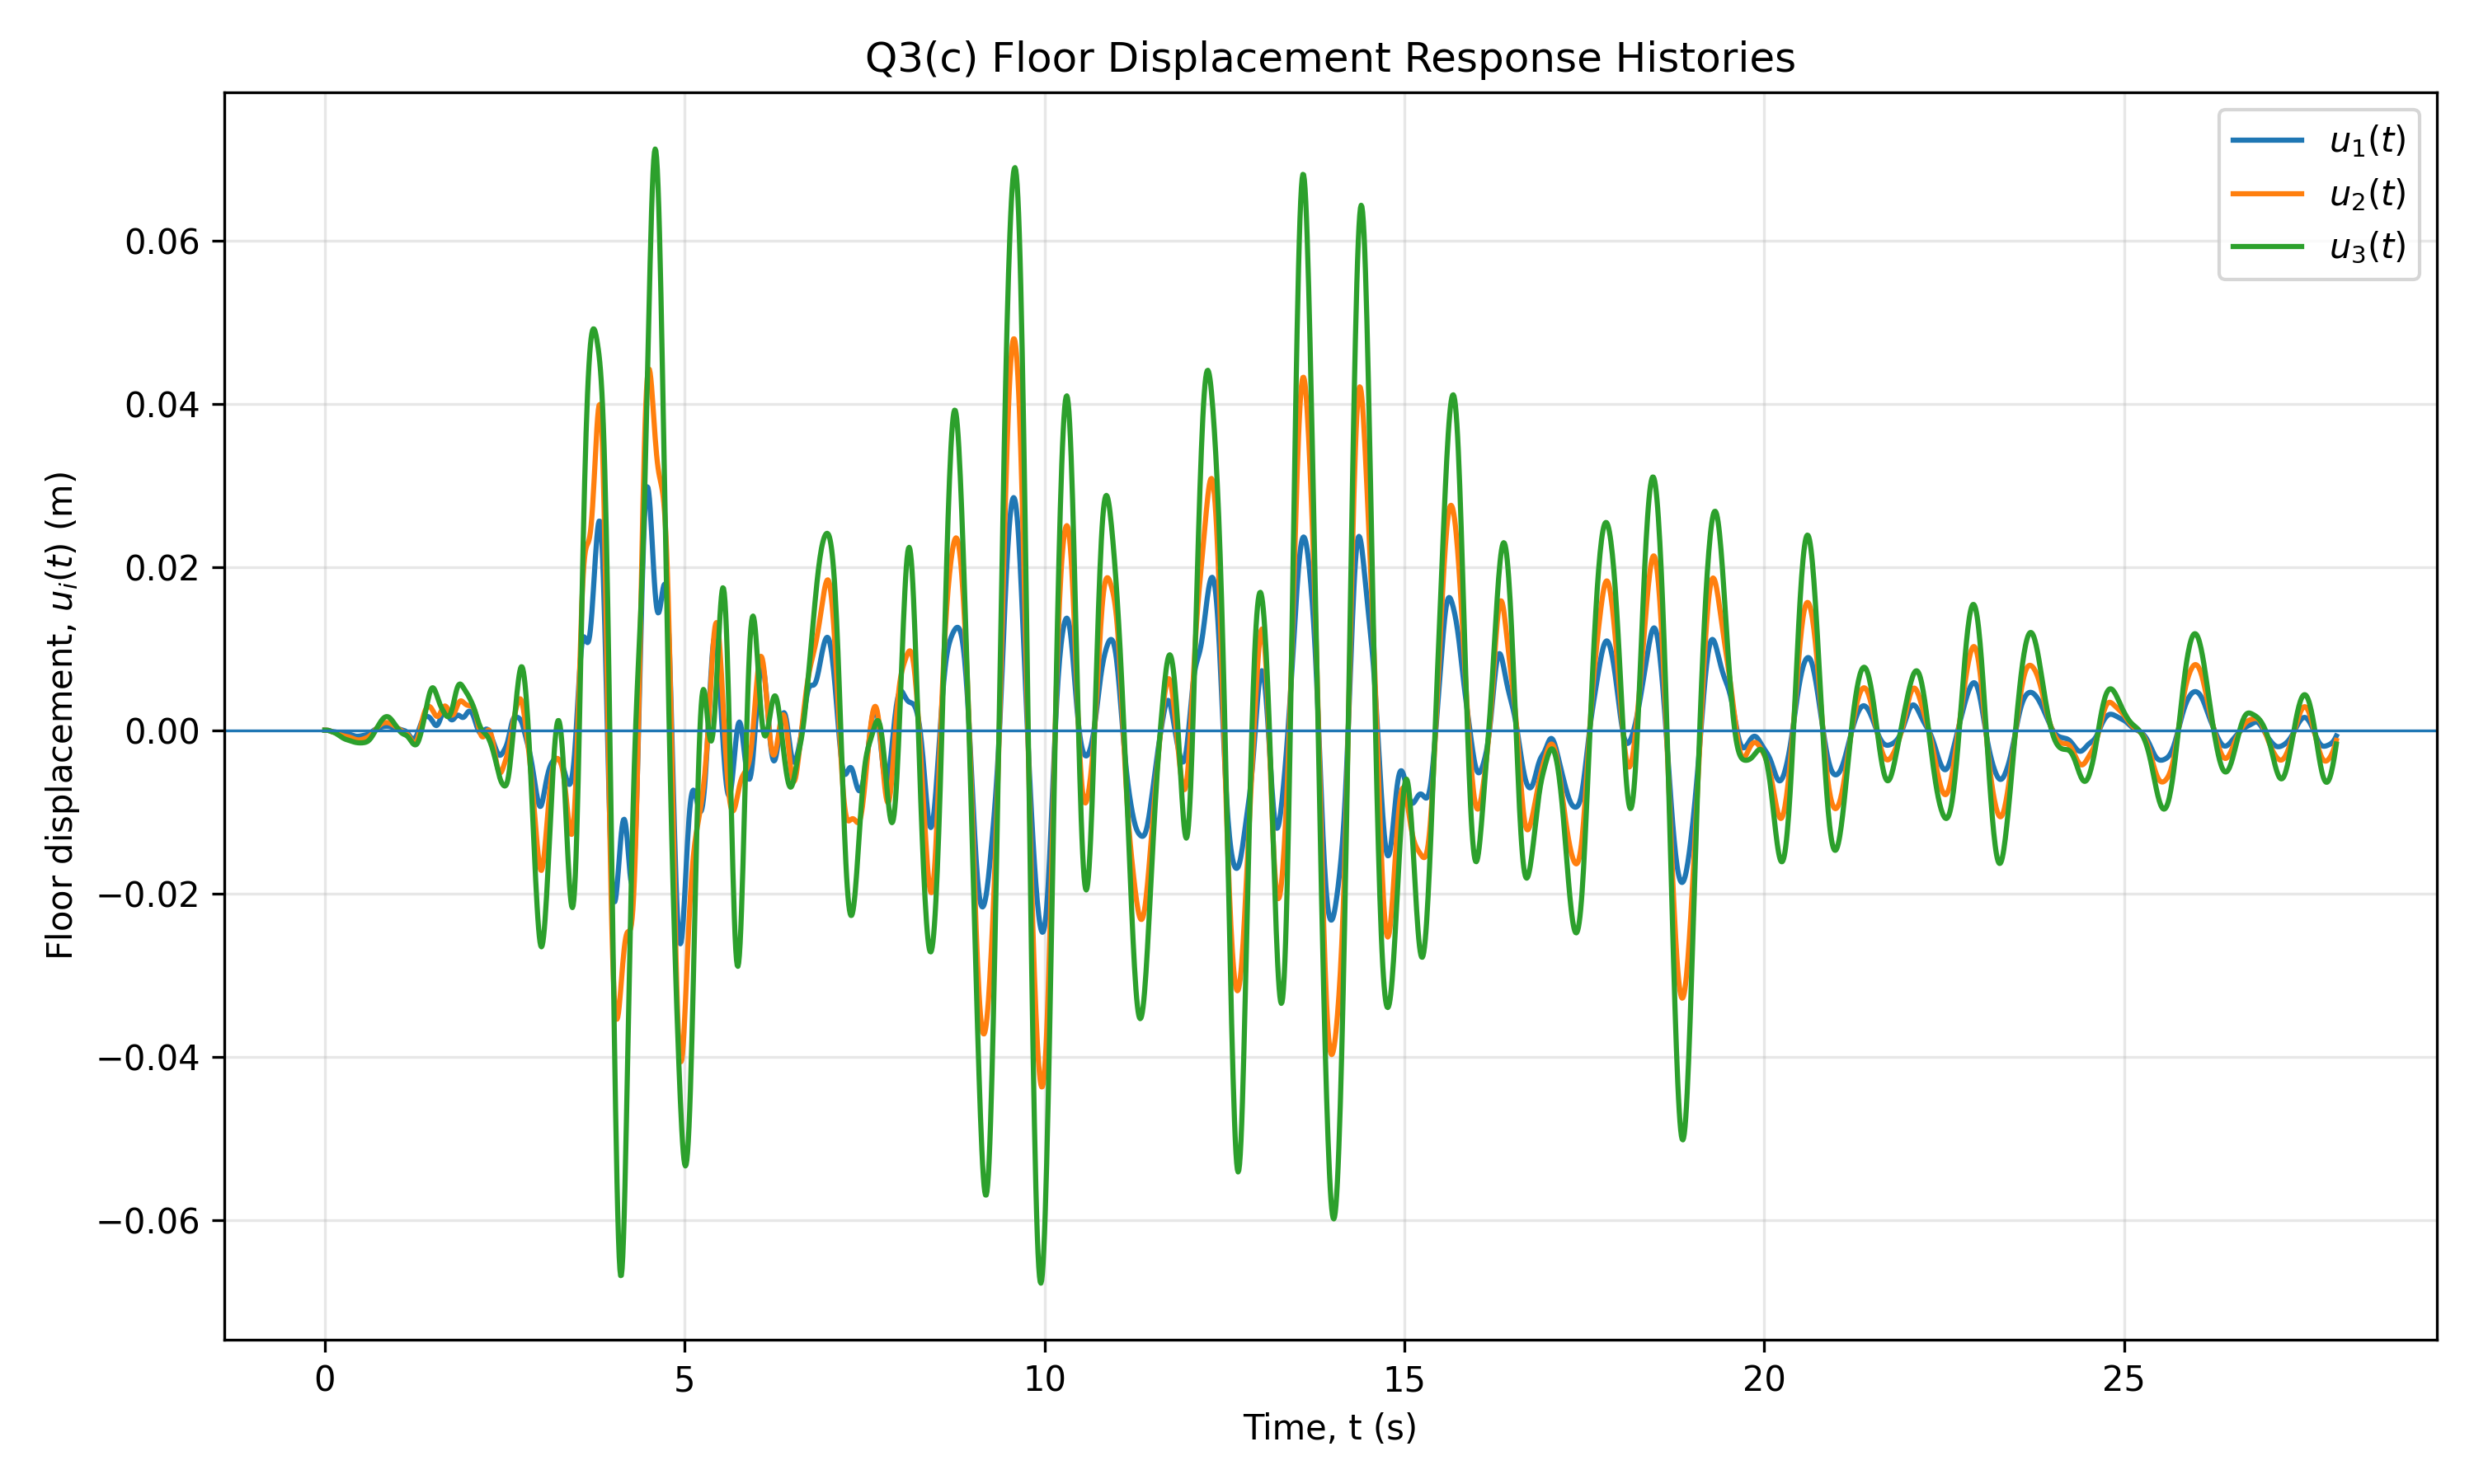
\includegraphics[width=0.92\textwidth]{../figures/Q3c_floor_displacement_histories.png}
\caption{Floor displacement response histories.}
\label{fig:q3c_displacements}
\end{figure}

\begin{figure}[H]
\centering
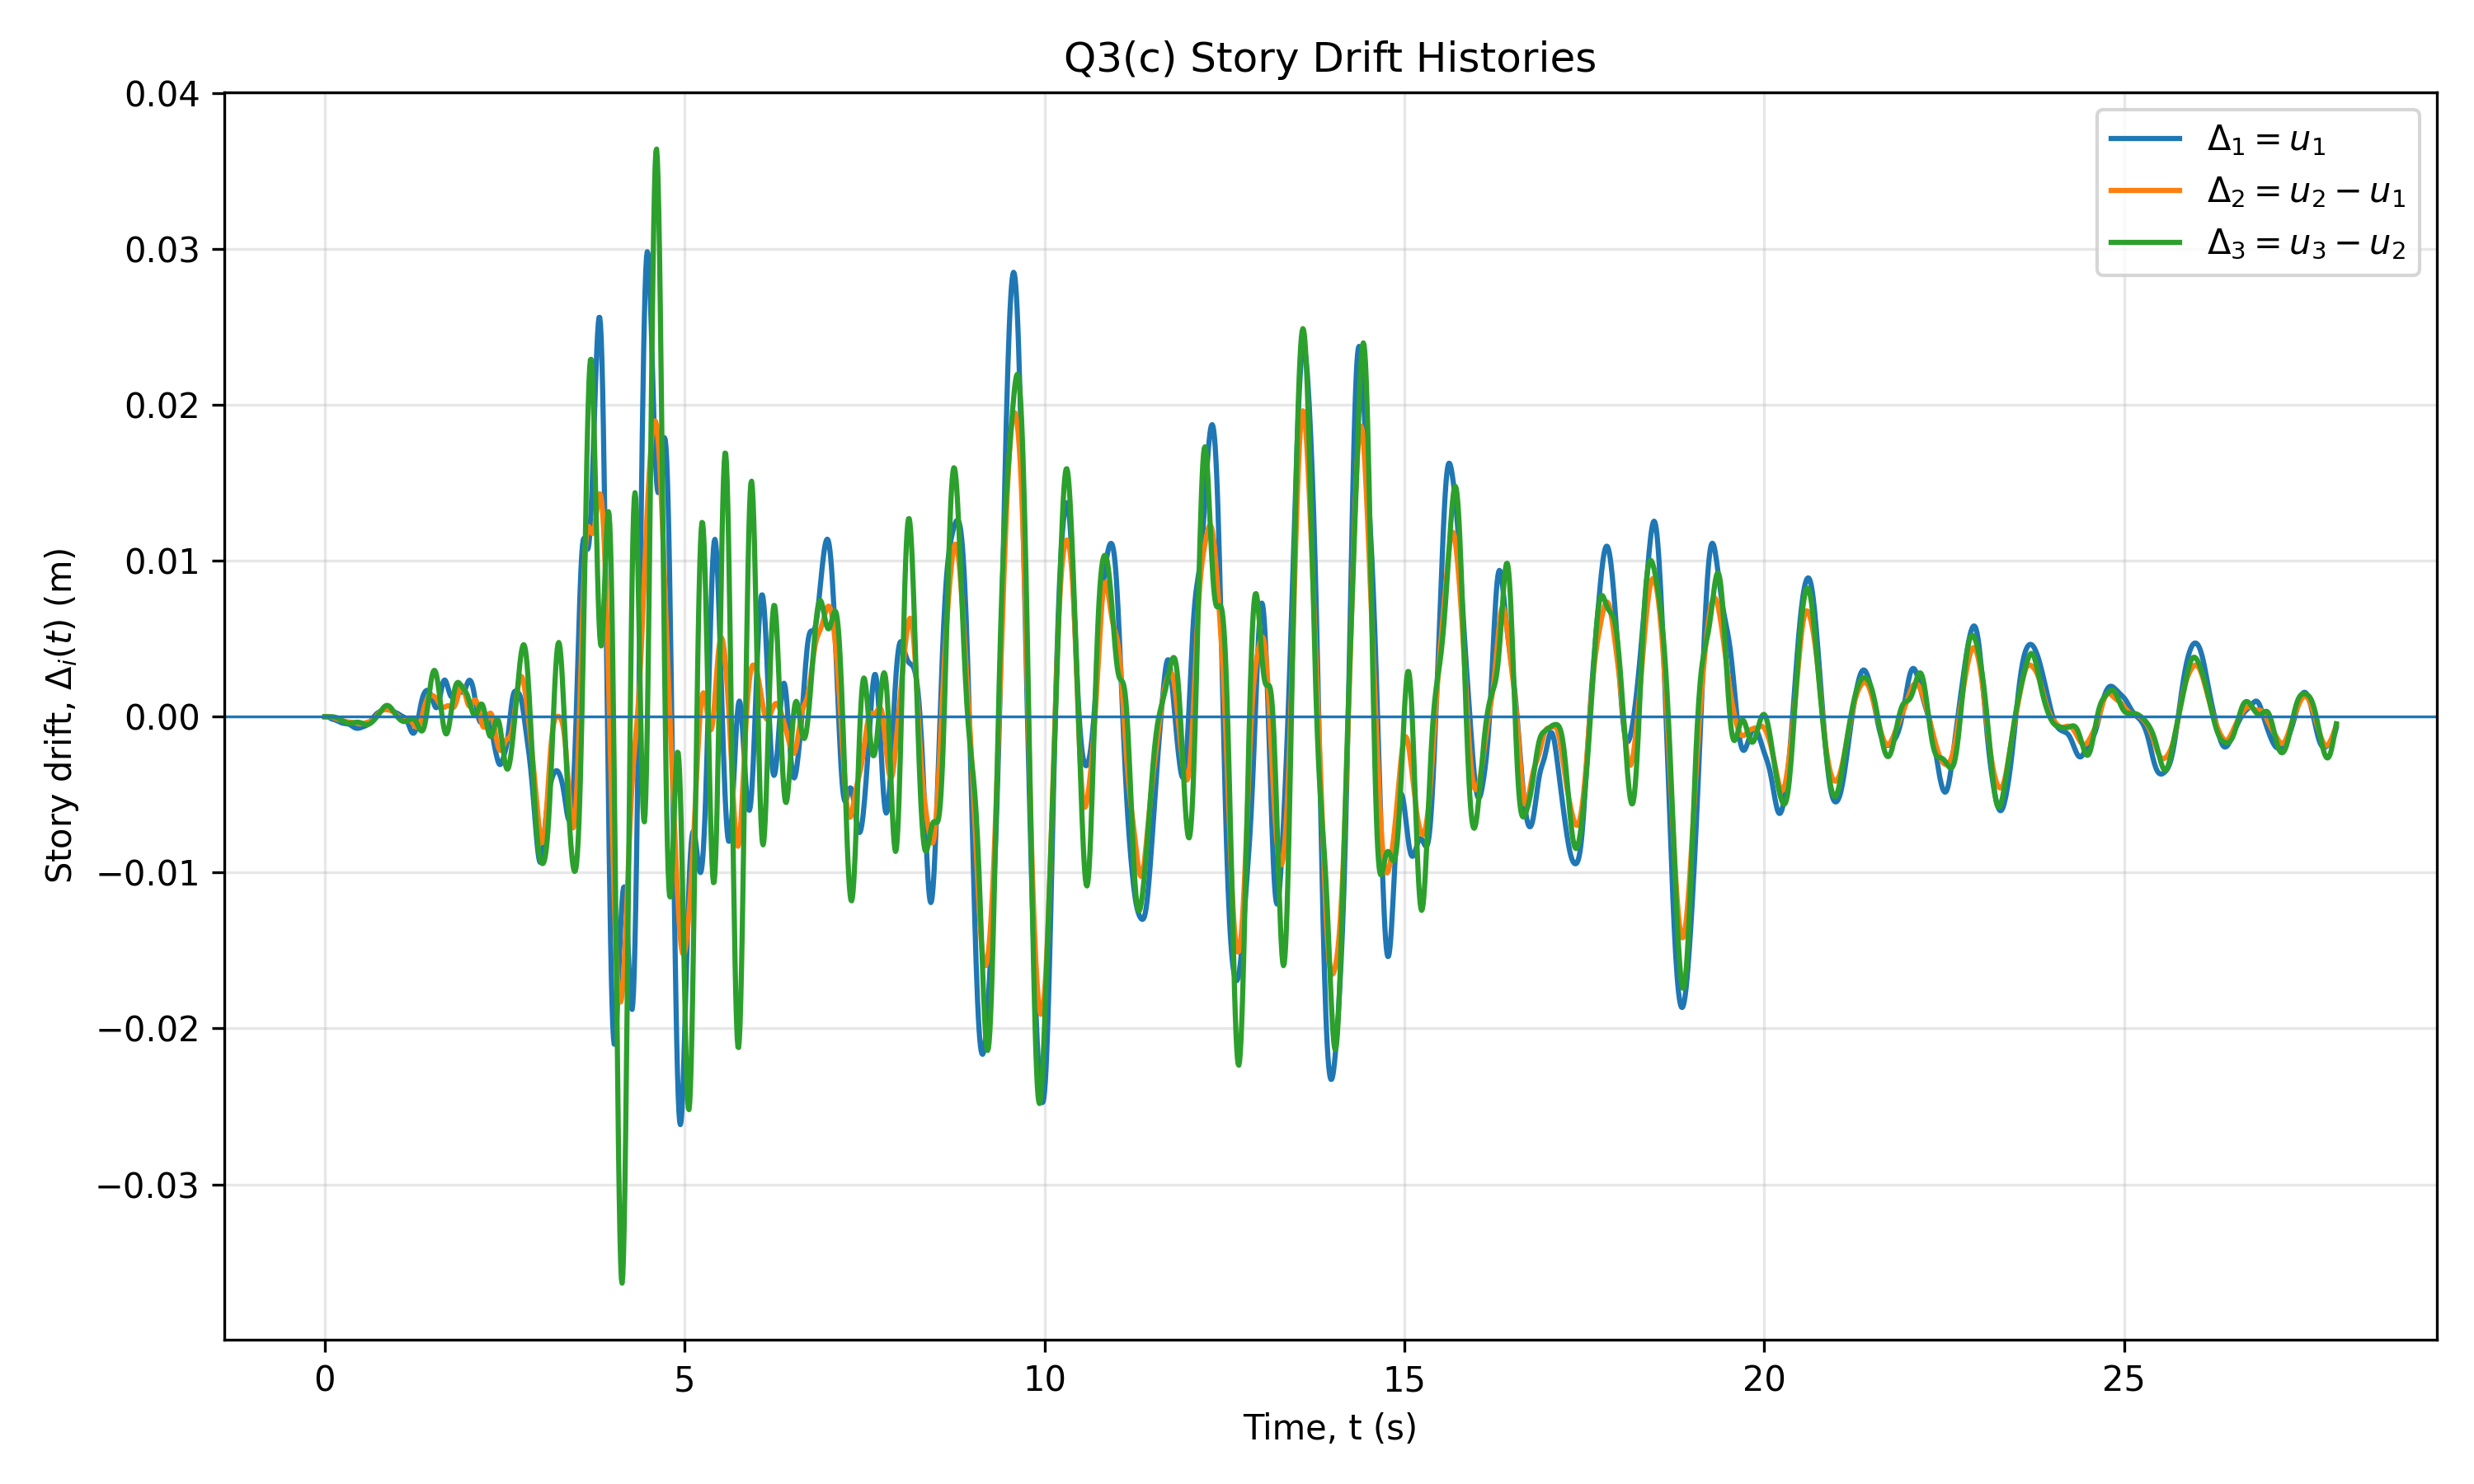
\includegraphics[width=0.92\textwidth]{../figures/Q3c_story_drift_histories.png}
\caption{Story drift histories.}
\label{fig:q3c_drifts}
\end{figure}

\subsection{Modal Floor Forces, Story Shears, and Base Shear}
For each mode, the signed modal floor-force vector is
\begin{equation}
\mathbf{f}_n(t)=\mathbf{s}_nA_n(t),
\end{equation}
where the signed modal-force pattern is
\begin{equation}
\mathbf{s}_n=\Gamma_n\,\mathbf{M}\,\boldsymbol{\phi}_n.
\end{equation}
Using the computed modal quantities, the three floor-force vectors and floor forces are
\begin{equation}
\mathbf{f}_1=\begin{bmatrix}9.869806\\13.104351\\19.993140\end{bmatrix}A_1(t),\quad
\mathbf{f}_2=\begin{bmatrix}7.376206\\4.465392\\-5.657809\end{bmatrix}A_2(t),\quad
\mathbf{f}_3=\begin{bmatrix}2.753988\\-2.569743\\0.664669\end{bmatrix}A_3(t).
\end{equation}

There are two methods to obtain the base shear response for each mode
Method 1, using the sum of modal floor forces:
\begin{equation}
V_{bn}(t)=\sum_{i=1}^{N}f_{in}(t)=\left(\sum_{i=1}^{N}s_{in}\right)A_n(t)
\end{equation}

Alternatively:
\begin{equation}
V_{bn}(t)=M_n^*A_n(t)
\end{equation}

Mode-by-mode base-shear modal equations are
\begin{equation}
V_{b1}(t)=\left(9.86980634+13.10435097+19.99313955\right)A_1(t)=42.96729686\,A_1(t),
\end{equation}
\begin{equation}
V_{b2}(t)=\left(7.37620601+4.46539241-5.65780890\right)A_2(t)=6.18378952\,A_2(t),
\end{equation}
\begin{equation}
V_{b3}(t)=\left(2.75398765-2.56974348+0.66466935\right)A_3(t)=0.84891352\,A_3(t).
\end{equation}

Verification (numeric) for each mode:
\begin{equation}
M_1^*=42.967297=\sum_{i=1}^{3}s_{i1},\quad
M_2^*=6.183790=\sum_{i=1}^{3}s_{i2},\quad
M_3^*=0.848914=\sum_{i=1}^{3}s_{i3}.
\end{equation}

 There are two methods to obtain the base overturning moment response for each mode
Method 1, using the sum of floor forces times heights:
\begin{equation}
M_{bn}(t)=\sum_{i=1}^{N}h_if_{in}(t)
\end{equation}

Define the static modal base moment coefficient:
\begin{equation}
M_{bn}^{st}=\sum_{i=1}^{N}h_is_{in}
\end{equation}
so that
\begin{equation}
M_{bn}(t)=M_{bn}^{st}A_n(t)
\end{equation}

The per-floor contributions ($h_i s_{in}$) and their sums are:
\begin{equation}
\begin{aligned}
&\text{Mode }n=1:\\
&\quad h_1 s_{11}=3.0\cdot 9.86980634=29.60941902,\\
&\quad h_2 s_{21}=6.0\cdot 13.10435097=78.62610582,\\
&\quad h_3 s_{31}=9.0\cdot 19.99313955=179.93825595,\\
&\quad \sum_{i=1}^3 h_i s_{i1}=288.17378079;\\
&\text{Mode }n=2:\\
&\quad h_1 s_{12}=3.0\cdot 7.37620601=22.12861803,\\
&\quad h_2 s_{22}=6.0\cdot 4.46539241=26.79235446,\\
&\quad h_3 s_{32}=9.0\cdot(-5.65780890)=-50.92028010,\\
&\quad \sum_{i=1}^3 h_i s_{i2}=-1.99930761;\\
&\text{Mode }n=3:\\
&\quad h_1 s_{13}=3.0\cdot 2.75398765=8.26196295,\\
&\quad h_2 s_{23}=6.0\cdot(-2.56974348)=-15.41846088,\\
&\quad h_3 s_{33}=9.0\cdot 0.66466935=5.98202415,\\
&\quad \sum_{i=1}^3 h_i s_{i3}=-1.17447378.
\end{aligned}
\end{equation}

Method 2, using the effective modal height:
\begin{equation}
M_{bn}(t)=h_n^*V_{bn}(t)
\end{equation}
Therefore,
\begin{equation}
M_{bn}(t)=h_n^*M_n^*A_n(t).
\end{equation}

The raw signed base-moment coefficients are
\begin{equation}
M_{b1}^{st}=288.173781,\quad M_{b2}^{st}=-1.999308,\quad M_{b3}^{st}=-1.174474.
\end{equation}
The corresponding effective modal heights are
\begin{equation}
h_1^*=6.706817,\quad h_2^*=-0.323314,\quad h_3^*=-1.383502.
\end{equation}
Thus, the mode-by-mode moment equations are
\begin{equation}
M_{b1}(t)=288.173781\,A_1(t)=6.706817\,M_1^*A_1(t),
\end{equation}
\begin{equation}
M_{b2}(t)=-1.999308\,A_2(t)=-0.323314\,M_2^*A_2(t),
\end{equation}
\begin{equation}
M_{b3}(t)=-1.174474\,A_3(t)=-1.383502\,M_3^*A_3(t).
\end{equation}
Numerical verification gives
\begin{equation}
M_{b1}^{st}\approx h_1^*M_1^*,\quad M_{b2}^{st}\approx h_2^*M_2^*,\quad M_{b3}^{st}\approx h_3^*M_3^*.
\end{equation}

The story shears are calculated from story stiffness and interstory drift:
\begin{equation}
V_1=k_1u_1,
\qquad
V_2=k_2(u_2-u_1),
\qquad
V_3=k_3(u_3-u_2).
\end{equation}

\begin{table}[H]
\centering
\caption{Maximum story shears.}
\begin{tabular}{cccc}
\toprule
Story & $\max|V_i|$ (kN) & Time (s) & Signed value (kN)\\
\midrule
1 & 190.88 & 4.48 & 190.88\\
2 & 125.56 & 13.59 & 125.56\\
3 & 116.51 & 4.61 & 116.51\\
\bottomrule
\end{tabular}
\label{tab:q3_story_shears}
\end{table}

Since $V_i$ are story shears rather than floor forces, the base overturning moment is obtained by integrating the story shear diagram over the building height. For equal story height $h_s=3\ \mathrm{m}$,
\begin{equation}
\boxed{
M_b(t)=3\left[V_1(t)+V_2(t)+V_3(t)\right]
}
\end{equation}

The maximum base responses are
\begin{equation}
\boxed{\max|V_b|=190.88\ \mathrm{kN}\quad \text{at}\quad t=4.48\ \mathrm{s}}
\end{equation}
\begin{equation}
\boxed{\max|M_b|=1120.93\ \mathrm{kNm}\quad \text{at}\quad t=9.58\ \mathrm{s}}
\end{equation}

\begin{figure}[H]
\centering
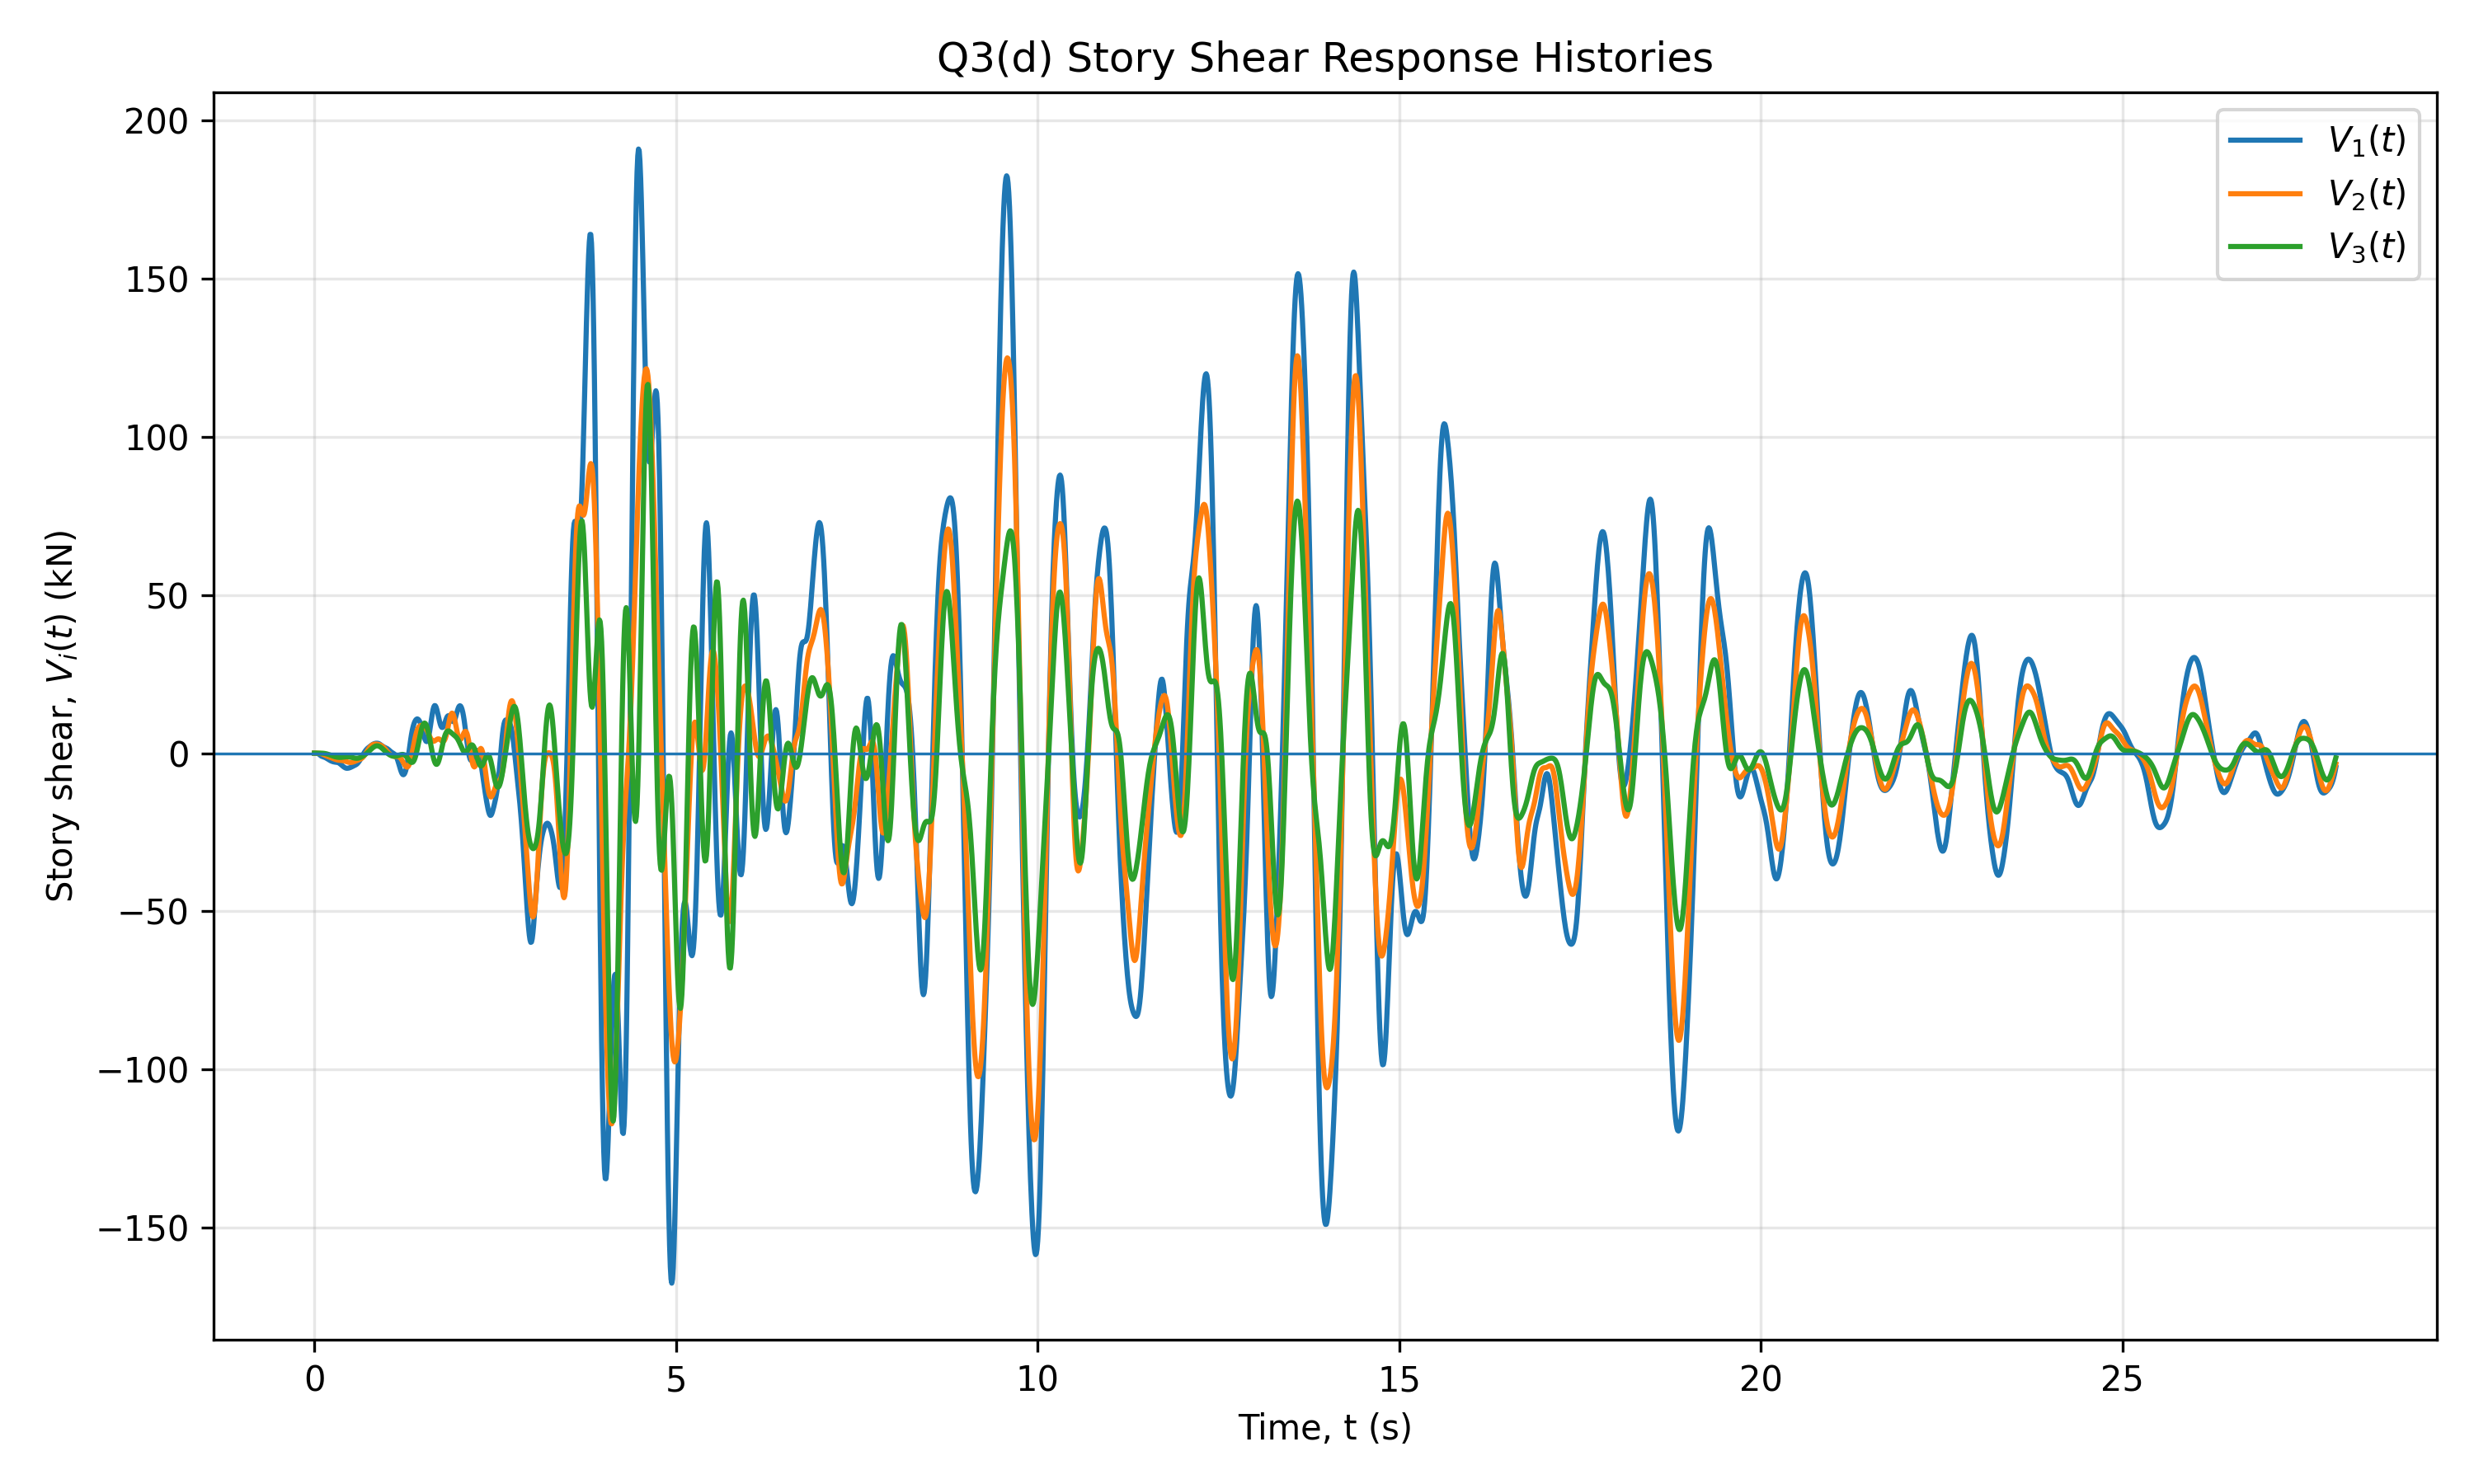
\includegraphics[width=0.92\textwidth]{../figures/Q3d_story_shear_histories.png}
\caption{Story shear response histories.}
\label{fig:q3d_story_shears}
\end{figure}

\begin{figure}[H]
\centering
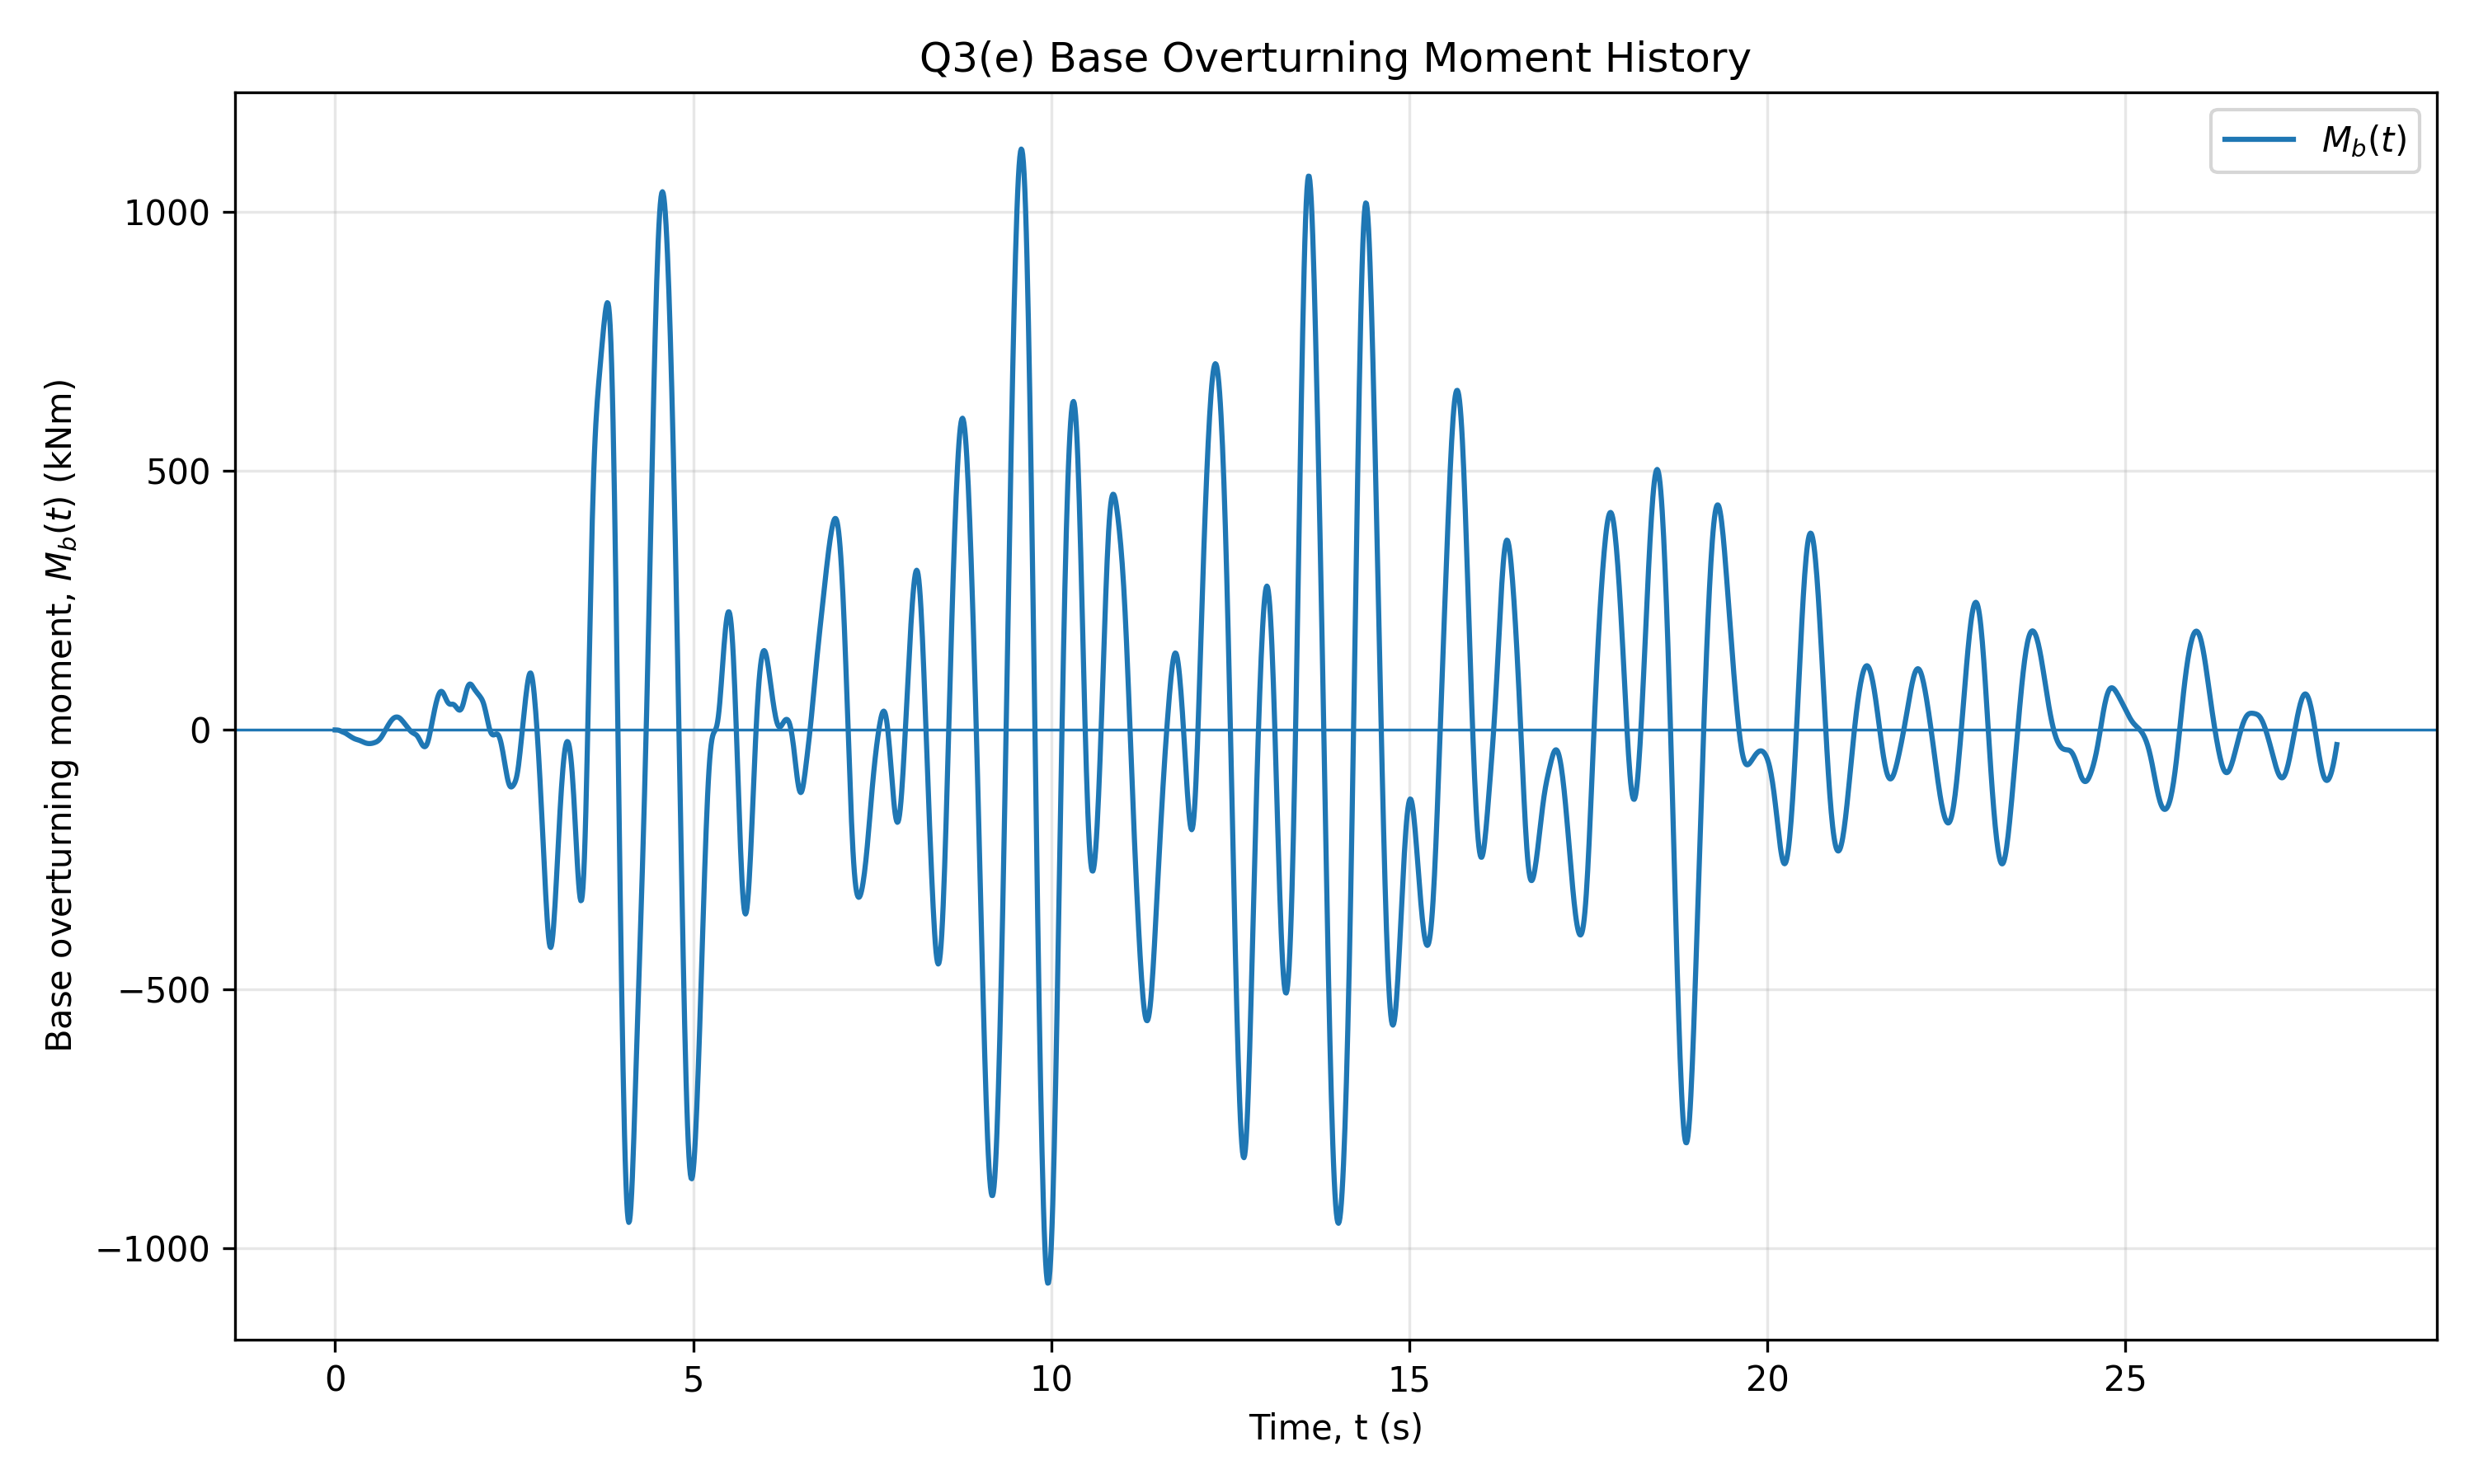
\includegraphics[width=0.92\textwidth]{../figures/Q3e_base_overturning_moment_history.png}
\caption{Base overturning moment history.}
\label{fig:q3e_moment}
\end{figure}

\subsection{Effective Modal Base Responses}
The effective modal mass is
\begin{equation}
M_n^*=\frac{L_n^2}{M_n},
\end{equation}
and the effective modal height is
\begin{equation}
h_n^*=\frac{\bm{\phi}_n^T\bm{M}\bm{h}}{L_n},
\qquad
\bm{h}=\begin{bmatrix}3&6&9\end{bmatrix}^T\ \mathrm{m}.
\end{equation}

\begin{table}[H]
\centering
\caption{Effective modal masses and heights.}
\begin{tabular}{cccc}
\toprule
Mode & $M_n^*$ (t) & Mass participation (\%) & $h_n^*$ (m)\\
\midrule
1 & 42.967 & 85.93 & 6.707\\
2 & 6.184 & 12.37 & -0.323\\
3 & 0.849 & 1.70 & -1.384\\
\bottomrule
\end{tabular}
\label{tab:q3_effective_modal}
\end{table}

The sum of the effective modal masses is
\begin{equation}
\sum_{n=1}^{3}M_n^*=50.000\ \mathrm{t},
\end{equation}
which is equal to the total physical mass of the structure. This confirms modal completeness for the three-degree-of-freedom system.

The total base shear and overturning moment time histories are assembled by summing the modal contributions at every time step:
\begin{equation}
V_b(t)=\sum_{n=1}^{3}M_n^*\,\omega_n^2\,D_n(t),
\qquad
M_b(t)=\sum_{n=1}^{3}h_n^*\,M_n^*\,\omega_n^2\,D_n(t).
\end{equation}
The peak of each modal contribution, evaluated at that mode's own maximum displacement, is
\begin{align}
V_{b1}^{\max} &= 42.967\,(8.573542)^2(0.05317)
              = 167.928\ \mathrm{kN} \quad (t=9.58\ \mathrm{s}),\\
V_{b2}^{\max} &= 6.184\,(19.537283)^2(0.03115)
              = 73.529\ \mathrm{kN}  \quad (t=4.45\ \mathrm{s}),\\
V_{b3}^{\max} &= 0.849\,(32.219905)^2(0.00641)
              = 5.650\ \mathrm{kN}   \quad (t=3.73\ \mathrm{s}).
\end{align}
These individual modal maxima occur at \emph{different} time instants and cannot be directly summed. Their combination is the basis for the RSA rules in Section~4.

At the instant of maximum total base shear, $t = 4.48$~s, the modal displacements read from the time history are
$D_1(4.48) = 0.03969303$~m,
$D_2(4.48) = 0.02793626$~m,
$D_3(4.48) = -0.00047677$~m,
giving
\begin{align}
V_{b1}(4.48) &= 42.967\,(8.573542)^2\,(0.03969303)
             = 125.364\ \mathrm{kN},\\
V_{b2}(4.48) &= 6.184\,(19.537283)^2\,(0.02793626)
             = 65.940\ \mathrm{kN},\\
V_{b3}(4.48) &= 0.849\,(32.219905)^2\,(-0.00047677)
             = -0.420\ \mathrm{kN},\\
V_b(4.48)   &= 125.364 + 65.940 - 0.420
             = 190.884\ \mathrm{kN}.
\end{align}

At the instant of maximum total overturning moment, $t = 9.58$~s, the modal displacements read from the time history are
$D_1(9.58) = 0.05317476$~m,
$D_2(9.58) = 0.00556213$~m,
$D_3(9.58) = 0.00098066$~m,
giving
\begin{align}
M_{b1}(9.58) &= 6.707\,(42.967)\,(8.573542)^2\,(0.05317476)
             = 1126.3687\ \mathrm{kNm},\\
M_{b2}(9.58) &= -0.323\,(6.184)\,(19.537283)^2\,(0.00556213)
             = -4.2447\ \mathrm{kNm},\\
M_{b3}(9.58) &= -1.384\,(0.849)\,(32.219905)^2\,(0.00098066)
             = -1.1957\ \mathrm{kNm},\\
M_b(9.58)   &= 1126.3687 - 4.2447 - 1.1957
             = 1120.9283\ \mathrm{kNm}
\end{align}

The maximum values of the combined time histories are:
\begin{equation}
\boxed{\max|V_b| = 190.88\ \mathrm{kN} \text{ at } t = 4.48\ \mathrm{s}}
\end{equation}
\begin{equation}
\boxed{\max|M_b| = 1120.93\ \mathrm{kNm} \text{ at } t = 9.58\ \mathrm{s}}
\end{equation}
These agree with the direct RHA results from parts~(d) and~(e) to within numerical roundoff, confirming that the effective modal parameter formulation is equivalent to direct modal superposition and that the three modes capture 100\% of the structural mass.
\pagebreak
% ------------------------------------------------------------
\section{Q4: Response Spectrum Analysis and Equivalent Static Procedure}
% ------------------------------------------------------------

\subsection{Construction of the 5\% Elastic Response Spectrum}

The 5\% elastic response spectrum was constructed by solving the linear elastic SDOF equation
\begin{equation}
\ddot{u}+2\xi\omega\dot{u}+\omega^2u=-\ddot{u}_g(t)
\end{equation}
for a range of natural periods. The spectral displacement is
\begin{equation}
S_d(T)=\max_t|u(t)|,
\end{equation}
and the pseudo-acceleration spectrum is
\begin{equation}
S_a(T)=\omega^2S_d(T).
\end{equation}

The spectral values at the structural modal periods are listed in Table~\ref{tab:q4a_modal_spectrum}.

\begin{table}[H]
\centering
\caption{5\% response spectrum ordinates at the structural modal periods.}
\begin{tabular}{cccc}
\toprule
Mode & $T_n$ (s) & $S_d$ (m) & $S_a$ (g)\\
\midrule
1 & 0.733 & 0.05314 & 0.39831\\
2 & 0.322 & 0.03121 & 1.21524\\
3 & 0.195 & 0.00667 & 0.70417\\
\bottomrule
\end{tabular}
\label{tab:q4a_modal_spectrum}
\end{table}

\begin{figure}[H]
\centering
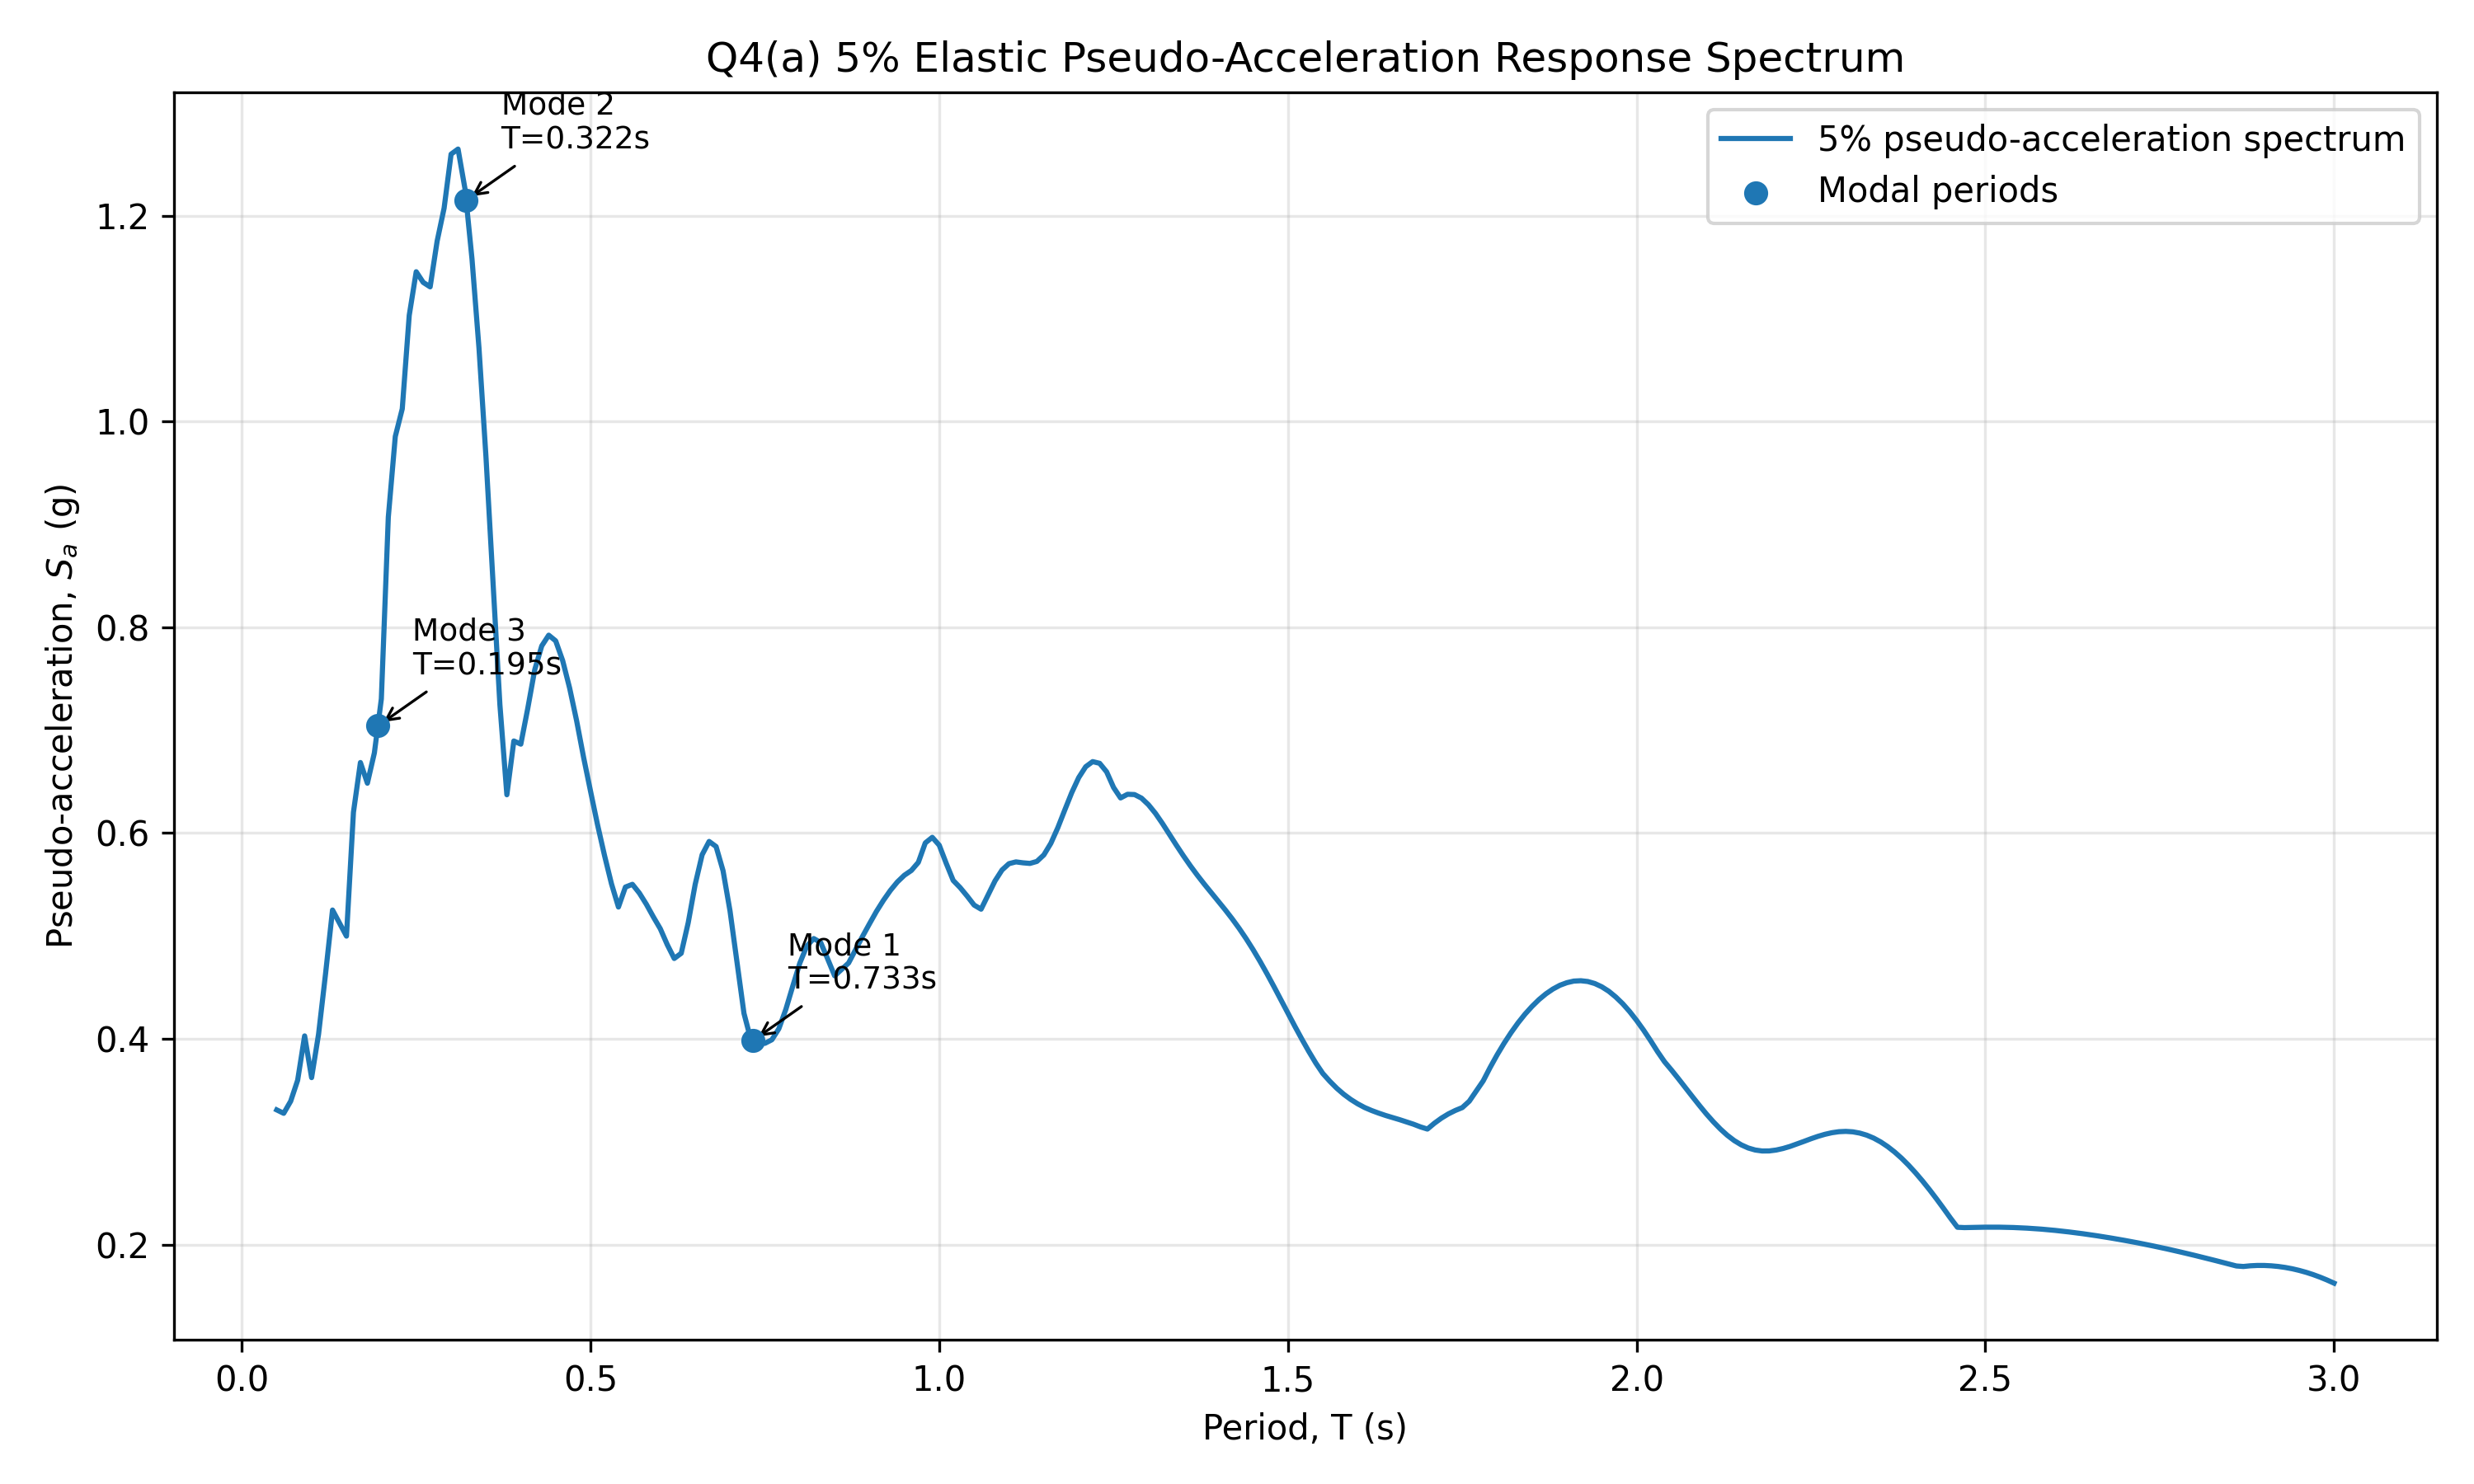
\includegraphics[width=0.92\textwidth]{../figures/Q4a_5percent_elastic_pseudo_acceleration_spectrum.png}
\caption{5\% elastic pseudo-acceleration response spectrum for the DIN95Y01 record.}
\label{fig:q4a_Sa}
\end{figure}

\begin{figure}[H]
\centering
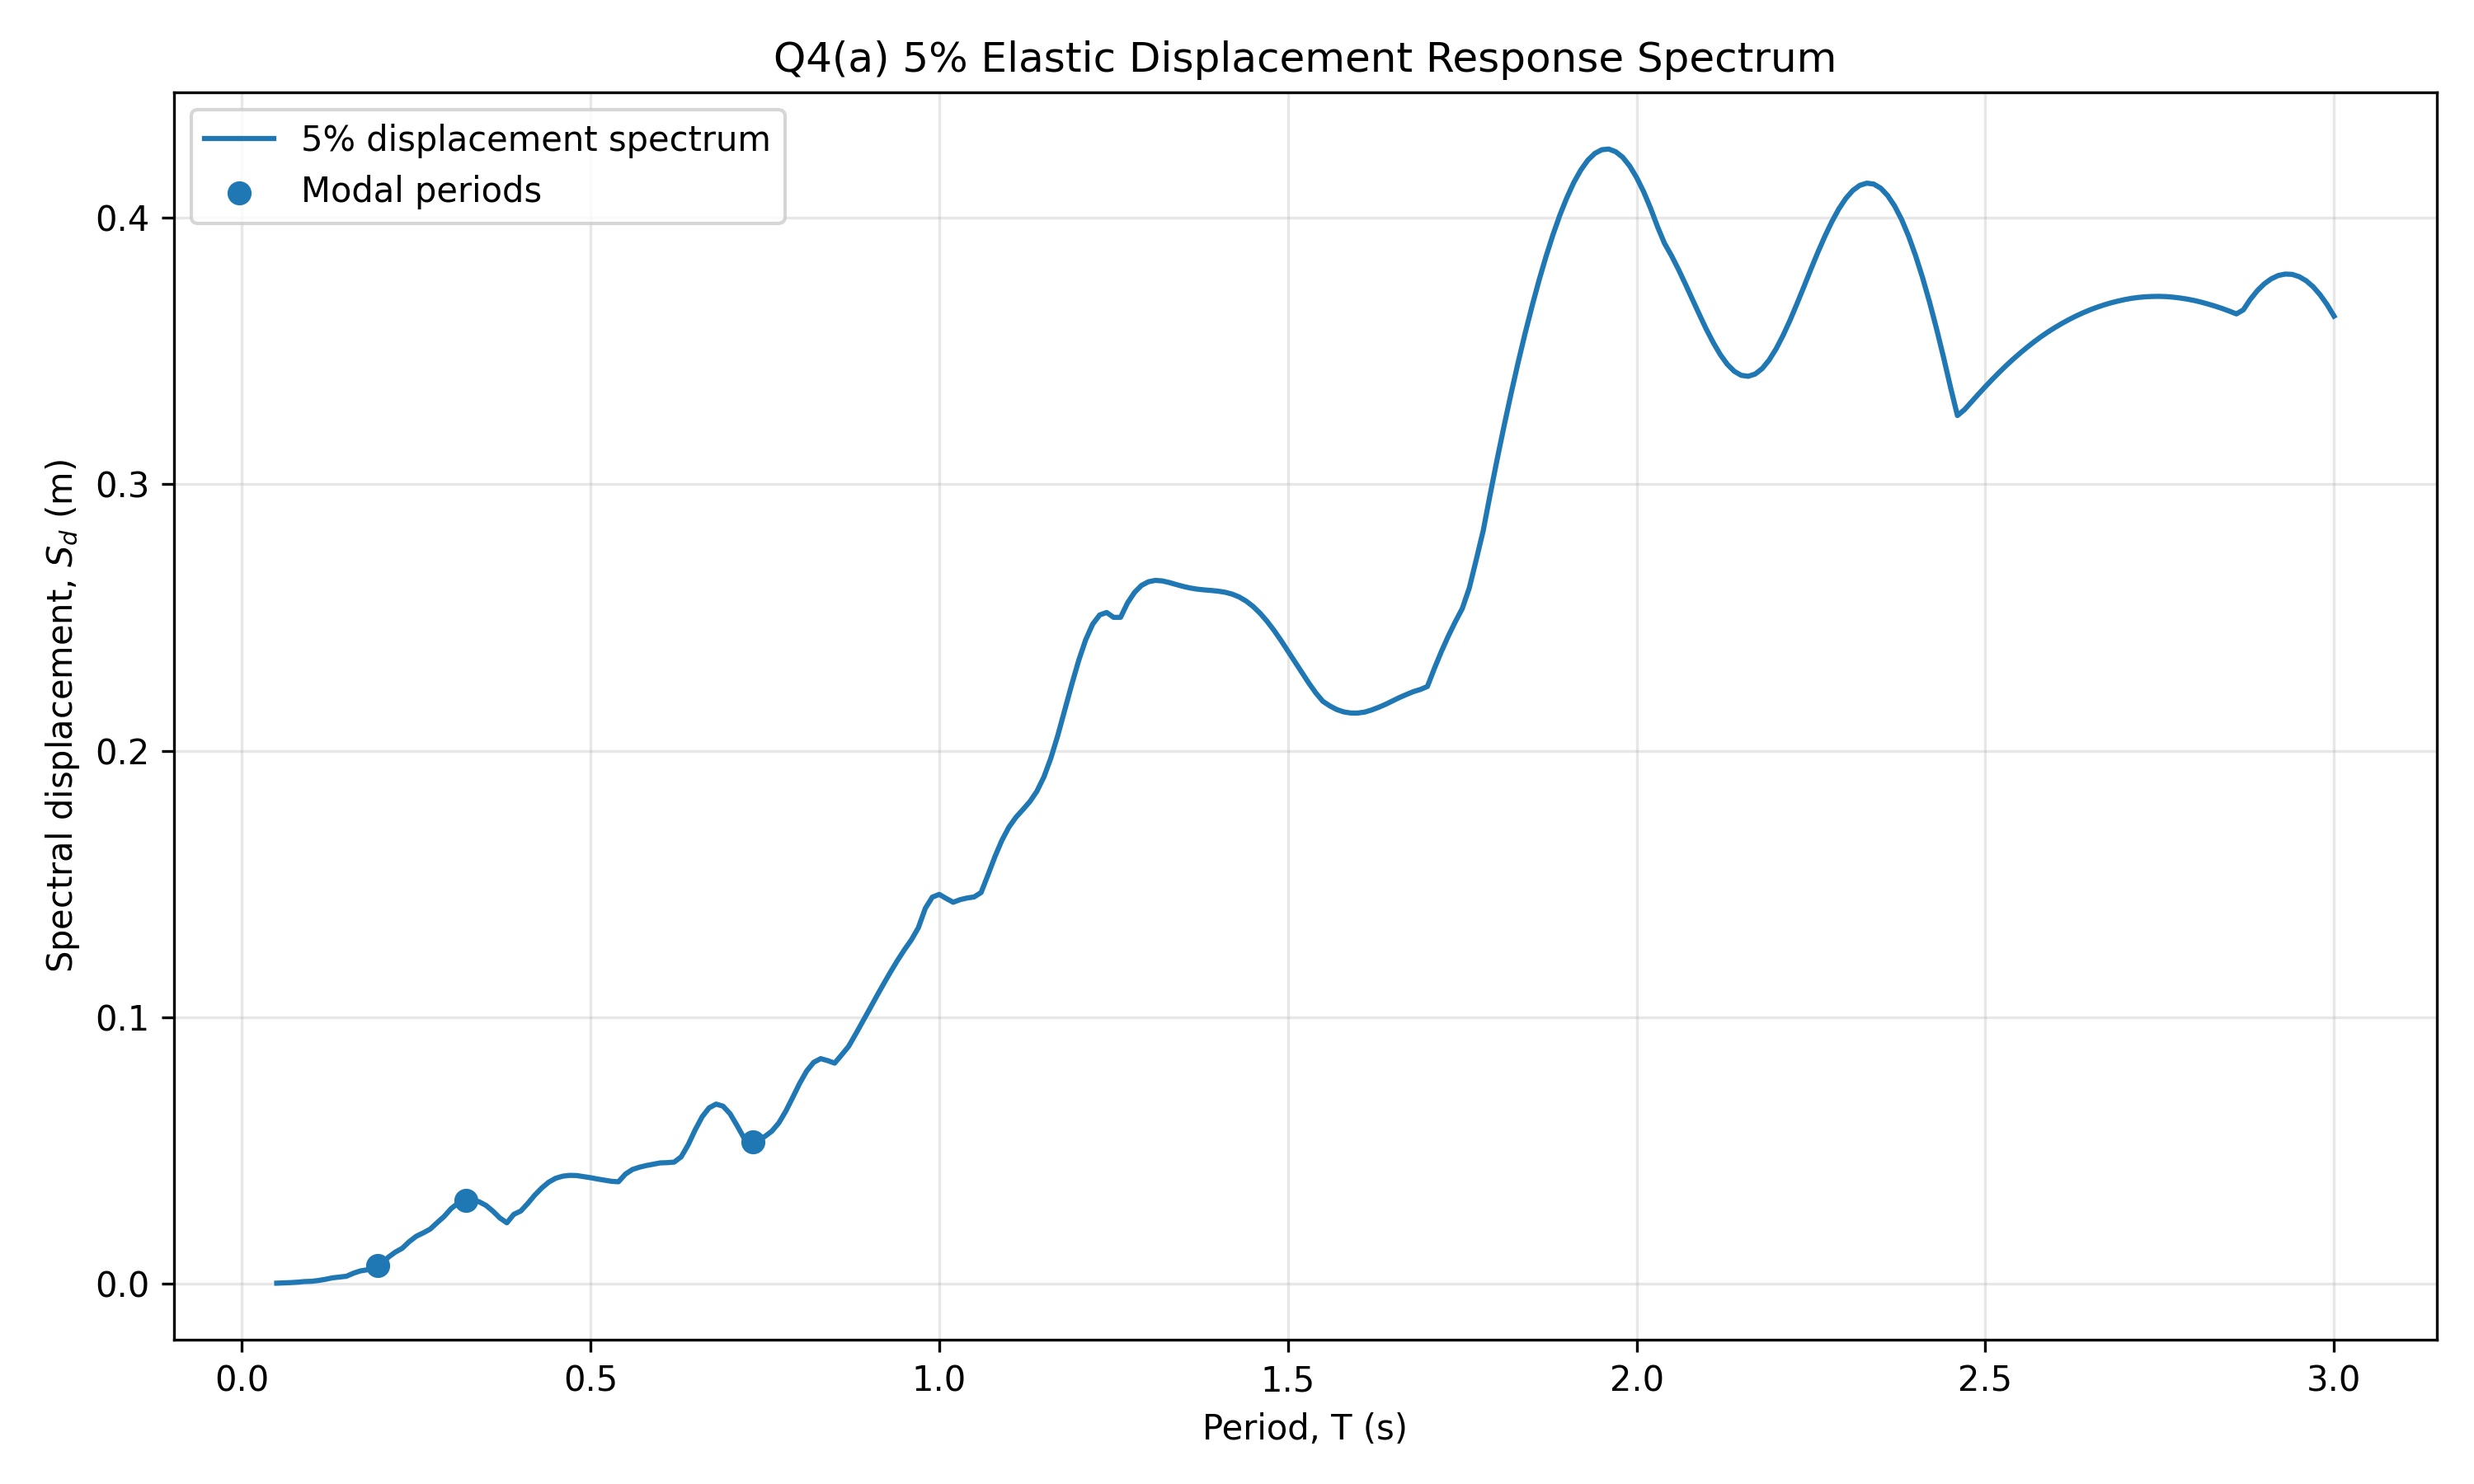
\includegraphics[width=0.92\textwidth]{../figures/Q4a_5percent_elastic_displacement_spectrum.png}
\caption{5\% elastic displacement response spectrum for the DIN95Y01 record.}
\label{fig:q4a_Sd}
\end{figure}

\subsection{Response Spectrum Analysis}

For each mode, the modal displacement contribution is
\begin{equation}
\bm{u}_n^{\max}=\bm{\phi}_n\Gamma_nS_{d,n}.
\end{equation}
Story shears are then obtained from modal story drifts, and the base overturning moment contribution is calculated using the story-shear relation
\begin{equation}
M_{b,n}=3(V_{1,n}+V_{2,n}+V_{3,n}).
\end{equation}

The modal responses are combined using ABSSUM, SRSS, and CQC. The CQC modal correlation coefficient is computed using the standard equal-damping expression.

\begin{table}[H]
\centering
\caption{RSA floor displacement maxima.}
\begin{tabular}{cccc}
\toprule
Floor & ABSSUM (m) & SRSS (m) & CQC (m)\\
\midrule
1 & 0.03865 & 0.02866 & 0.02880\\
2 & 0.05686 & 0.04736 & 0.04746\\
3 & 0.08290 & 0.07180 & 0.07165\\
\bottomrule
\end{tabular}
\label{tab:q4b_displacements}
\end{table}

\begin{table}[H]
\centering
\caption{RSA story shear maxima.}
\begin{tabular}{cccc}
\toprule
Story & ABSSUM (kN) & SRSS (kN) & CQC (kN)\\
\midrule
1 & 247.39 & 183.39 & 184.35\\
2 & 156.65 & 130.72 & 130.54\\
3 & 150.11 & 103.28 & 102.53\\
\bottomrule
\end{tabular}
\label{tab:q4b_shears}
\end{table}

\begin{table}[H]
\centering
\caption{RSA base overturning moment maxima.}
\begin{tabular}{cc}
\toprule
Combination rule & $M_b$ (kNm)\\
\midrule
ABSSUM & 1157.56\\
SRSS & 1125.90\\
CQC & 1125.57\\
\bottomrule
\end{tabular}
\label{tab:q4b_moment}
\end{table}

\subsection{Comparison of RHA and RSA}

\begin{table}[H]
\centering
\caption{Comparison of RHA and RSA response quantities.}
\resizebox{\textwidth}{!}{%
\begin{tabular}{llrrrrrrr}
\toprule
Response & Unit & RHA & RSA ABSSUM & Diff. (\%) & RSA SRSS & Diff. (\%) & RSA CQC & Diff. (\%)\\
\midrule
$u_1$ & m & 0.02983 & 0.03865 & 29.60 & 0.02866 & -3.92 & 0.02880 & -3.42\\
$u_2$ & m & 0.04795 & 0.05686 & 18.58 & 0.04736 & -1.23 & 0.04746 & -1.02\\
$u_3$ & m & 0.07121 & 0.08290 & 16.42 & 0.07180 & 0.84 & 0.07165 & 0.63\\
$V_1$ & kN & 190.88 & 247.39 & 29.60 & 183.39 & -3.92 & 184.35 & -3.42\\
$V_2$ & kN & 125.56 & 156.65 & 24.76 & 130.72 & 4.11 & 130.54 & 3.97\\
$V_3$ & kN & 116.51 & 150.11 & 28.84 & 103.28 & -11.36 & 102.53 & -12.00\\
$M_b$ & kNm & 1120.93 & 1157.56 & 3.27 & 1125.90 & 0.44 & 1125.57 & 0.41\\
\bottomrule
\end{tabular}%
}
\label{tab:q4c_comparison}
\end{table}

ABSSUM is consistently conservative because it assumes that the modal maxima occur simultaneously and with the most unfavorable signs. SRSS and CQC are much closer to RHA because the modal periods are reasonably separated and modal correlation is limited. The largest deviations occur in story shear responses, particularly in the upper story, which is expected because local force quantities are more sensitive to higher-mode effects than global displacement and overturning moment quantities.

\subsection{Equivalent Static Lateral Force Procedure}

For the equivalent static procedure, the design spectrum provided in the assignment is used. The design spectral acceleration is
\begin{equation}
A(T)=
\begin{cases}
0.4+0.6\dfrac{T}{0.15}, & 0\leq T\leq 0.15,\\[6pt]
1.0, & 0.15<T\leq 0.60,\\[6pt]
\left(\dfrac{0.6}{T}\right)^{0.8}, & T>0.60.
\end{cases}
\end{equation}

Using the fundamental period
\begin{equation}
T_1=0.732858\ \mathrm{s}>0.60\ \mathrm{s},
\end{equation}
the spectral acceleration is
\begin{equation}
A(T_1)=\left(\frac{0.6}{0.732858}\right)^{0.8}=0.852129g.
\end{equation}

The total mass is
\begin{equation}
M_{\mathrm{tot}}=50\ \mathrm{t},
\end{equation}
and the base shear is
\begin{equation}
\boxed{V_b=M_{\mathrm{tot}}A(T_1)g=417.83\ \mathrm{kN}}.
\end{equation}

The floor forces are distributed as
\begin{equation}
F_i=V_b\frac{m_ih_i}{\sum_jm_jh_j}.
\end{equation}
Since
\begin{equation}
\sum_jm_jh_j=20(3)+15(6)+15(9)=285\ \mathrm{t\,m},
\end{equation}
the floor forces are given in Table~\ref{tab:q4d_forces}.

\begin{table}[H]
\centering
\caption{Equivalent static floor forces.}
\begin{tabular}{cccc}
\toprule
Floor & Mass (t) & Height (m) & $F_i$ (kN)\\
\midrule
1 & 20.0 & 3.0 & 87.96\\
2 & 15.0 & 6.0 & 131.95\\
3 & 15.0 & 9.0 & 197.92\\
\bottomrule
\end{tabular}
\label{tab:q4d_forces}
\end{table}

The base overturning moment from the equivalent static forces is
\begin{equation}
M_b=\sum_iF_ih_i,
\end{equation}
which gives
\begin{equation}
\boxed{M_b=2836.82\ \mathrm{kNm}}.
\end{equation}

\subsection{Final Comparison of RHA, RSA, and ESLFP}

\begin{table}[H]
\centering
\caption{Comparison of RHA, RSA, and ESLFP base responses.}
\begin{tabular}{lrrrr}
\toprule
Method & $V_b$ (kN) & $M_b$ (kNm) & $V_b$ diff. from RHA (\%) & $M_b$ diff. from RHA (\%)\\
\midrule
RHA & 190.88 & 1120.93 & 0.00 & 0.00\\
RSA ABSSUM & 247.39 & 1157.56 & 29.60 & 3.27\\
RSA SRSS & 183.39 & 1125.90 & -3.92 & 0.44\\
RSA CQC & 184.35 & 1125.57 & -3.42 & 0.41\\
ESLFP & 417.83 & 2836.82 & 118.90 & 153.08\\
\bottomrule
\end{tabular}
\label{tab:q4e_final_comparison}
\end{table}

The RHA result is the direct time-domain response to the DIN95Y01 record. The SRSS and CQC RSA results agree closely with the RHA base responses, especially for base overturning moment. ABSSUM was conservative, while the equivalent static procedure produced substantially larger base shear and overturning moment because it was based on the prescribed design spectrum rather than the record-specific response spectrum. Furthermore, SRSS/CQC Mb values (1125.90/1125.57 kNm) are within 0.5% of the RHA value (1120.93 kNm). Therefore, ESLFP represents a more conservative design-level estimate, while RHA and RSA reflect the demand from the assigned ground motion.
\pagebreak
% ------------------------------------------------------------
\section{Conclusion}
% ------------------------------------------------------------

The flexurally rigid-beam model produced a fundamental period of approximately $0.733\ \mathrm{s}$, whereas the finite-beam condensed model produced a significantly longer period of approximately $1.380\ \mathrm{s}$, demonstrating the effect of beam flexibility on lateral stiffness. Modal response history analysis showed that the first mode dominates the displacement response, with an effective modal mass participation of approximately 85.93\%. The record-based RSA results using SRSS and CQC were close to the RHA results, particularly for the base overturning moment. ABSSUM was conservative, while the equivalent static procedure produced substantially larger base shear and overturning moment because it was based on the prescribed design spectrum.

The numerical calculations were carried out using a Python implementation based on NumPy and Matplotlib. The script performs eigenvalue analysis, Newmark average-acceleration integration, response spectrum construction, modal response spectrum analysis, and equivalent static force calculations. The generated CSV files and plots were used to prepare the tables and figures in this report.

\end{document}
